%% Submissions for peer-review must enable line-numbering 
%% using the lineno option in the \documentclass command.
%%
%% Preprints and camera-ready submissions do not need 
%% line numbers, and should have this option removed.
%%
%% Please note that the line numbering option requires
%% version 1.1 or newer of the wlpeerj.cls file.


\documentclass[fleqn,10pt,lineno]{wlpeerj} % for journal submissions
%\documentclass[fleqn,10pt]{wlpeerj} % for preprint submissions


%\newcommand{\rr}{${\mathcal{R}}$}
\usepackage{amssymb}
\usepackage{amsmath}
\usepackage{upgreek}
\usepackage[]{fontenc}
\usepackage{color}
\usepackage{bm}
\usepackage[english]{babel}
\usepackage{graphicx}
\usepackage{tikz}
\usetikzlibrary{positioning}
\usepackage{ifthen}
\usepackage{xstring}
\usepackage{afterpage}
%\usepackage[hidelinks]{hyperref}
\usepackage{changepage}
\usepackage[colorlinks=true, allcolors=blue, pdfborder={0 0 0}]{hyperref}
\usepackage{soul}


% ==============

% ========================================================================================
% ========================================================================================
\usepackage[utf8]{inputenc}
\DeclareFixedFont{\ttb}{T1}{txtt}{bx}{n}{9} % for bold
\DeclareFixedFont{\ttm}{T1}{txtt}{m}{n}{9}  % for normal
% Defining colors
\usepackage{color}
\definecolor{deepblue}{rgb}{0,0,0.5}
\definecolor{deepred}{rgb}{0.6,0,0}
\definecolor{deepgreen}{rgb}{0,0.5,0}
\usepackage{listings}
\usepackage{textcomp} 
\usepackage[T1]{fontenc}
% for upquotes
\newcommand\pythonstyle{\lstset{
  language=Python,
  backgroundcolor=\color{white}, %%%%%%%
  % basicstyle=\ttm,
  basicstyle=\footnotesize,
  numbers=right,
  stepnumber=1,
  otherkeywords={self},            
  keywordstyle=\ttb\color{deepblue},
  emph={MyClass,__init__},          
  emphstyle=\ttb\color{deepred},    
  stringstyle=\color{deepgreen},
  commentstyle=\color{red},  %%%%%%%%
  frame=tb,                         
  showstringspaces=false,
  upquote=true,
  %obeytabs=true,
  tabsize=2
}}

% Python environment
\lstnewenvironment{python}[1][]
{
\pythonstyle
\lstset{#1}
}
{}

% Python for external files
\newcommand\pythonexternal[2][]{{
\pythonstyle
\lstinputlisting[#1]{#2}}}

% Python for inline
\newcommand\pythoninline[1]{{\pythonstyle\lstinline!#1!}}

\def\ContinueLineNumber{\lstset{firstnumber=last}}
% ========================================================================================
% ========================================================================================

\newcommand{\floor}[1]{\left \lfloor #1 \right \rfloor}
\newcommand{\round}[1]{\left \lfloor #1 \right \rceil }
\newcommand{\ceil}[1]{\left \lceil #1 \right \rceil }
\newcommand{\Fig}[1]{Fig.~\ref{#1}}
%\newcommand{\Fig}[1]{Figure~\ref{#1}}
\newcommand{\Figs}[1]{Figs.~\ref{#1}}
%\newcommand{\Figs}[1]{Figures~\ref{#1}}
\newcommand{\Sec}[1]{Section~\ref{#1}}
\newcommand{\Secs}[1]{Sections~\ref{#1}}
\newcommand{\Chap}[1]{Chapter~\ref{#1}}
\newcommand{\Chaps}[1]{Chapters~\ref{#1}}
\newcommand{\Tab}[1]{Table~\ref{#1}}
\newcommand{\Tabs}[1]{Tables~\ref{#1}}
\newcommand{\Eqn}[1]{Eqn.~\ref{#1}}
\newcommand{\Eqns}[1]{Eqns.~\ref{#1}}
\newcommand{\InEqn}[1]{Inequality~(\ref{#1})}
\newcommand{\InEqns}[1]{Inequalities~(\ref{#1})}
\newcommand{\Center}[1]{\textcolor{white}{.}\hfill#1\hfill\textcolor{white}{.}}
\newcommand{\ang}{$\textrm\AA$}
\newcommand{\new}[1]{#1}
\newcommand{\New}[1]{#1}
\newcommand{\old}[1]{}
%\newcommand{\o}[1]{\old{#1}}
\newcommand{\n}[1]{{\textbf{\color{red}#1}}}
%\newcommand{\n}[1]{{\hl{#1}}}
\newcommand{\we}{I~}

\usepackage{xspace}

\newcommand{\gname}{BackMAP}
\newcommand{\pname}{\textsc{\gname}\xspace}
\newcommand{\code}[1]{\texttt{#1}\xspace}

\usepackage[cal=cm,scrscaled=1.05]{mathalfa} % This is for \mathcal{}, particularly \mathcal{R}
\DeclareMathAlphabet\mathbfcal{OMS}{cmsy}{b}{n} % for boldface mathcal: \mathbfcal{}
\newcommand{\rr}{$\mathcal{R}$\xspace}

\def\kt{k_{\rm B}T}

\def\beq{\begin{equation}}
\def\eeq{\end{equation}}
\def\bea{\begin{eqnarray}}
\def\eea{\end{eqnarray}}

\def\cal#1{\mathcal{#1}}
\def\eqq#1{Eq.~(\ref{#1})}
\def\eq#1{(\ref{#1})}
\def\av#1{\langle #1 \rangle}

\def\f#1{Fig.~\ref{#1}}
\def\ff#1{Figs.~\ref{#1}}

\def\s#1{Section~\ref{#1}}

\def\c#1{~\cite{#1}}


%\newcommand{\c}[1]{\citep{#1}}

\newcommand{\figdir}{../figures}

\title{The Back\n{MAP} Python Module: How a Simpler Ramachandran Number Can Simplify the Life of a Protein Simulator}


\author[1,*]{Ranjan V. Mannige}
%\author[1,2,*]{Ranjan V. Mannige}
%\affil[1]{~KPMG, Atlanta, CA 30309, U.S.A.}
\affil[1]{~Multiscale Institute, Berkeley Lake, GA 30092, U.S.A.}
\affil[*]{~ranjanmannige@gmail.com}

%\keywords{Ramachandran number, Multi-angle Picture, MAP, Protein structure}

\begin{abstract}
Protein backbones occupy diverse conformations, but compact metrics to describe such conformations and transitions between them have been missing. This report re-introduces the Ramachandran number (\rr) as a residue-level structural metric that could simply the life of anyone contending with large numbers of protein backbone conformations (e.g., ensembles from NMR and trajectories from simulations). Previously, the Ramachandran number (\rr) was introduced using a complicated \n{closed form}, which made the Ramachandran number difficult to implement. This report discusses a much simpler closed form of \rr that makes it much easier to calculate, thereby making it easy to implement. Additionally, this report discusses how \rr dramatically reduces the dimensionality of the protein backbone, thereby making it ideal for simultaneously interrogating large number of protein structures. For example, two hundred distinct conformations can easily be described in one graphic using \rr (rather than two hundred distinct Ramachandran plots). Finally, a new Python-based backbone analysis tool -- \pname -- is introduced that reiterates how \rr can be used as a simple and succinct descriptor of protein backbones and their dynamics.
\end{abstract}

\begin{document}

\flushbottom
\maketitle
\thispagestyle{empty}

\section*{Introduction}

\begin{figure}[b!]
\centering
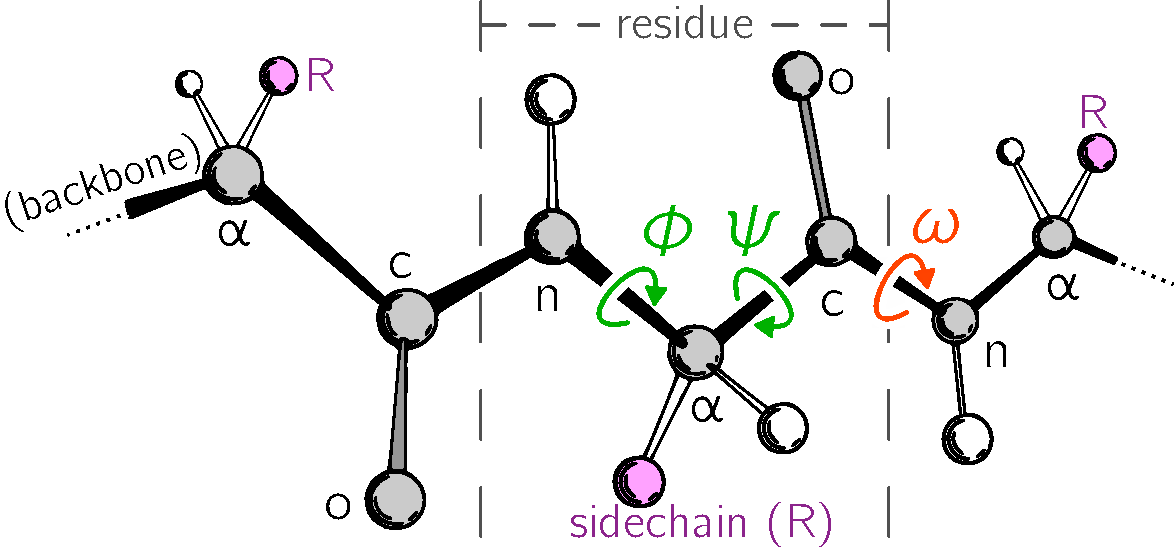
\includegraphics[width=0.4\linewidth]{backmap_fig1.pdf}
\caption{\textbf{Backbone conformational degrees of freedom} dominantly depend on the dihedral angles $\phi$ and $\psi$ (green), and to a smaller degree depend on the third dihedral angle ($\omega$; red) as well as bond lengths and angles (unmarked). \label{fig:intro}} 
\end{figure}

Proteins are a class of biomolecules unparalleled in their functionality \citep{Berg2006}. A natural protein may be thought of as a linear chain of amino acids, each normally sourced from a repertoire of 20 naturally occurring amino acids. 
%Its exact sequence of amino acids (its primary sequence) dictates much about the final conformation fo a protein. E.g., a protein of a specific sequence may repeatedly fold into (or assume) a certain three-dimensional conformation \citep{Berg2006}. 
Proteins are important partially because of the structures that they access: the conformations (conformational ensemble) that a protein assumes determines the functions available to that protein. However, all proteins are dynamic: even stable proteins undergo long-range motions in its equilibrium state; i.e., they have substantial diversity in their conformational ensemble \citep{James2003,James2003a,Oldfield2005,Tokuriki2009,Schad2011,Vertessy2011,Mannige2014b}. Additionally, a number of proteins undergo conformational transitions, without which they may not properly function. Finally, some proteins -- intrinsically disordered proteins -- display massive disorder whose conformations dramatically change over time \citep{Uversky2003, Fink2005, Midic2009, Espinoza-Fonseca2009, Uversky2010, Tompa2011, Sibille2012, Kosol2013, Dunker2013, Geist2013, Baruah2015}, and whose characteristic structures are still not well-understood \citep{Beck2008}.

Large-scale changes in a protein occur due to changes in protein backbone conformations. %\footnote{Sidechain conformational changes alone, while correlated in space and time -- see \cite{DuBay2011} -- can not alone contribute to the change in a protein fold/conformation.}. 
\Fig{fig:intro} is a cartoon representation of a peptide/protein backbone, with the backbone bonds themselves represented by darkly shaded bonds. \cite{Ramachandran1963} had recognized that the backbone conformational degrees of freedom available to an amino acid (residue) $i$ is almost completely described by only two dihedral angles: $\phi_i$ and $\psi_i$ (\Fig{fig:intro}, green arrows). %A third dihedral angle, $\omega_i$, is primarily planar at $180^\circ$; \cite{Pauling1951a,Pauling1951}]\footnote{See \Fig{fig:intro}a. For any amino acid $i$, $\phi_i$, $\psi_i$ and $\omega_i$ respectively involve the four atoms $\{\mathrm{C}_\mathrm{-1}, \mathrm{N}, \mathrm{C}\upalpha, \mathrm{C}\}$, $\{\mathrm{N}, \mathrm{C}\upalpha, \mathrm{C}, \mathrm{N}_\mathrm{+1}\}$, and  $\{\mathrm{C}\upalpha_\mathrm{-1}, \mathrm{C_{-1}}, \mathrm{N},\mathrm{C}\upalpha\}$.The central bond involving $\omega_i$ describes the amide bond connecting residues $(i-1)$ and $i$. An alternative $\omega_i$ involves the connection between residues $i$ and $(i+1)$, where the four relevant atoms are $\{\mathrm{C}\upalpha, \mathrm{C}, \mathrm{N_{+1}},\mathrm{C}\upalpha_{+1}\}$.}. 
\n{Today, Ramachandran plots are used to qualitatively describe protein backbone conformations}.

The Ramachandran plot is recognized as a powerful tool for two reasons: 1) it serves as a map for structural `correctness' \citep{Laskowski1993,Hooft1997,Laskowski2003}, since many regions within the Ramachandran plot space are energetically not permitted \citep{Momen2017}; and 2) it provides a qualitative snapshot of the structure of a protein \citep{Berg2006,Alberts2002,Subramanian2001,Lovell2003}. For example, particular regions within the Ramachandran plot indicate the presence of particular secondary locally-ordered structures such as the $\upalpha$-helix and $\upbeta$-sheet (see \Fig{fig:ramaintro}a).

While the Ramachandran plot has been useful as a measure of protein backbone conformation, it is not popularly used to assess structural dynamism and transitions (unless specific knowledge exists about whether a particular residue is believed to undergo a particular structural transition). This is because of the two-dimensionality of the plot: describing the behavior of every residue involves tracking its position in two-dimensional ($\phi$,$\psi$) space. For example, a naive description of positions of a peptide in a Ramachandran plot (\Fig{fig:ramaintro}b) needs more annotations for a per-residue analysis of the peptide backbone's structure. Given enough residues, it would be impractical to track the position of each residue within a plot. This is compounded with time, as each point in (b) becomes a curve (c), further confounding the situation. The possibility of picking out previously unseen conformational transitions and dynamism becomes a logistical impracticality. As indicated above, this impracticality arises primarily from the fact that the Ramachandran plot is a two-dimensional map.

\begin{figure*}[t!]
\begin{adjustwidth}{-1in}{0in} % Comment out/remove adjustwidth environment if table fits in text column.
\centering
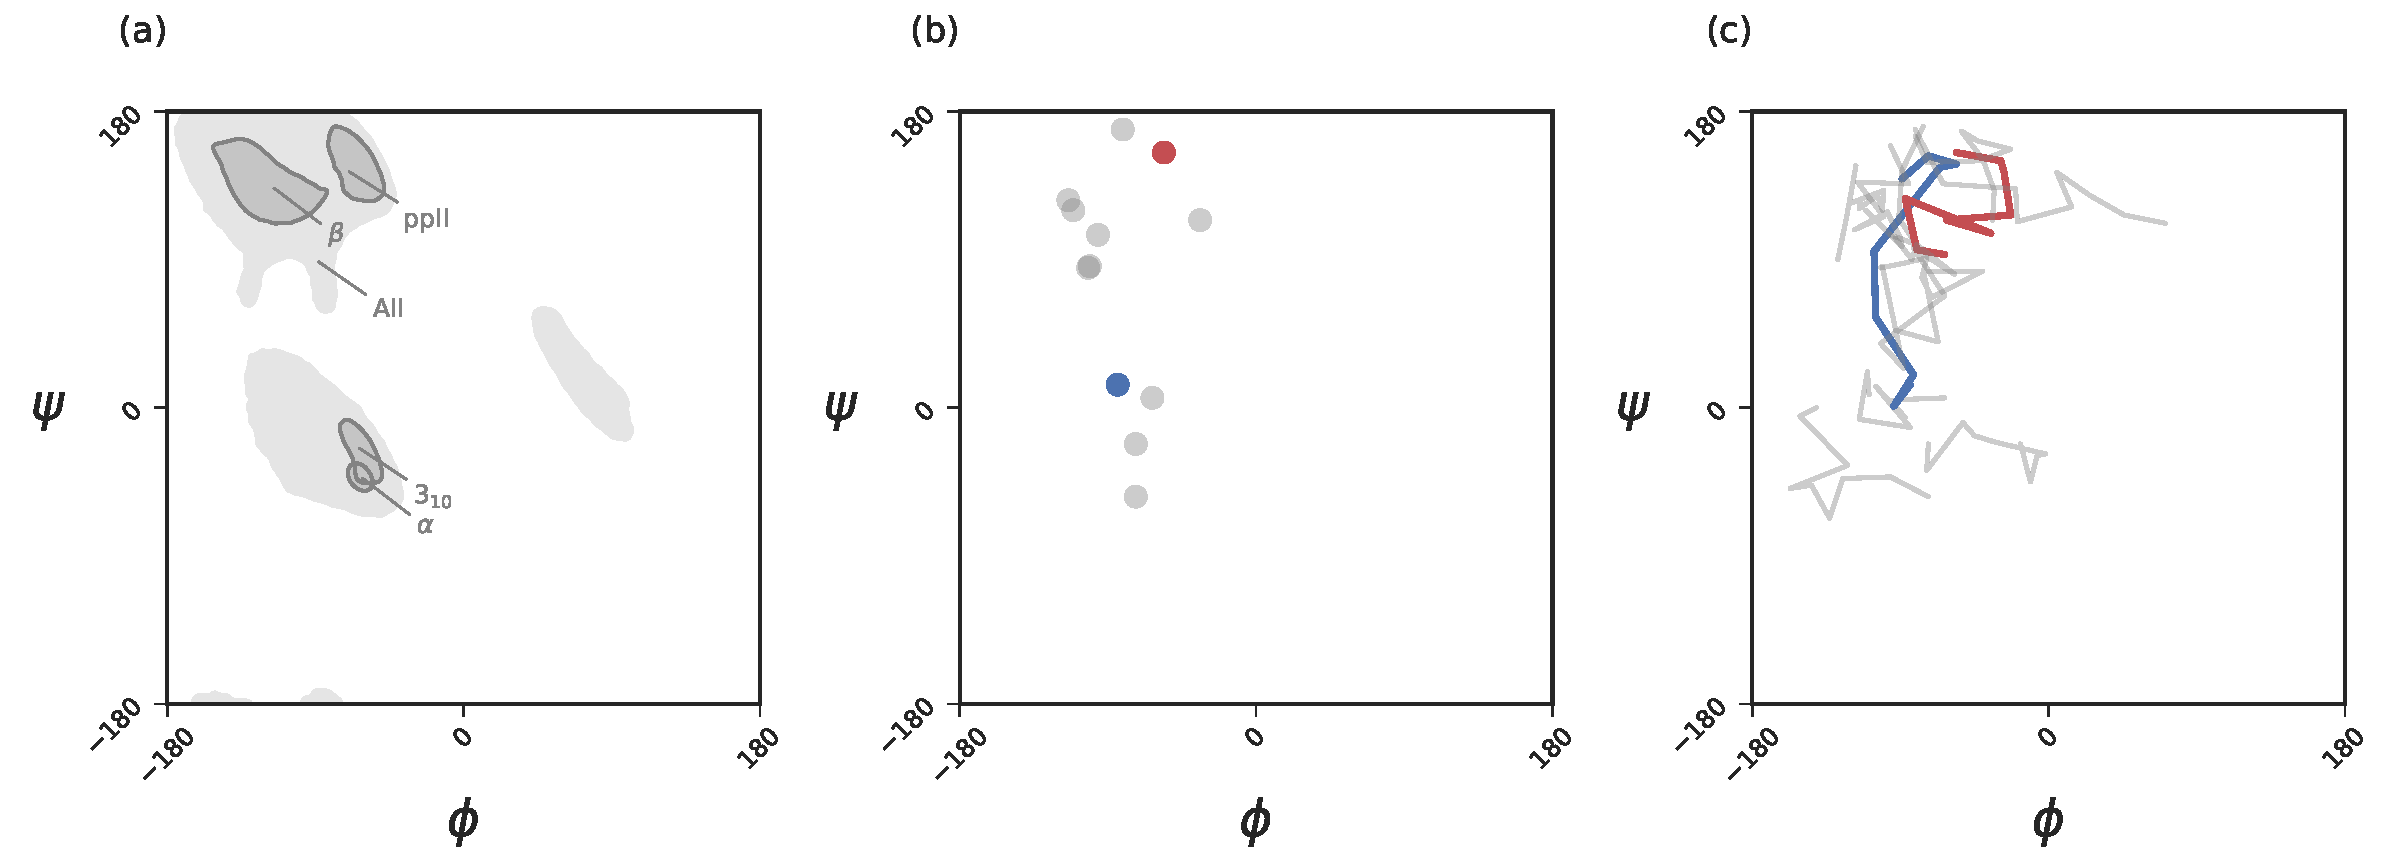
\includegraphics[width=1.0\linewidth]{backmap_fig2.pdf}
\caption{\n{Ramachandran plots allow for the per-residue representation of backbone conformation. Panel (a) represents regions in the plot that are occupied by backbones describing particular regular secondary structures. Panel (b) represents the positions of a 11 residue peptide that describe, with one dot per residue. Panel (c) represents a seven-frame trajectory, where each residue's backbone traces a line, with } While the Ramachandran plot is useful for getting a {\it qualitative} sense of peptide backbone structure (a, \n{b}), it is not a convenient representation for exploring peptide backbone dynamics (c). {\footnotesize Secondary structure keys used here and throughout the document: `$\alpha$' -- $\upalpha$-helix, `$3_{10}$' -- $3_{10}$-helix, `$\beta$' -- $\upbeta$-sheet/extension, `$\textrm{ppII}$' -- polyproline II helix.}\label{fig:ramaintro}} 
\end{adjustwidth}
\end{figure*}

For example, tracking changes in protein trajectory is either overly detailed or overly holistic: an example of an overly detailed study is the tracking on exactly one or a few atoms over time (this already poses a problem, since we would need to know exactly which atoms are expected to partake in a transition); an example of a holistic metric is the radius of gyration (this also poses a problem, since we will never know which residues contribute to a change in radius of gyration without additional interrogation). % While these metrics are heavily used by the molecular dynamics community, the change in these metrics over time only provides a general sense that something in the structure is changing. These metrics, however, can not provide any more residue-level details than that. 
With our understanding of protein dynamics undergoing a new \n{renaissance} -- especially due to intrinsically disordered proteins and allostery -- having hypothesis-agnostic yet detailed (residue-level) metrics of protein structure has become even more relevant. 
Consequently, there has been no single compact descriptor of protein structure. This impedes the na{\"i}ve or hypothesis-free exploration of new trajectories/ensembles. %\footnote{Of course, if prior knowledge (or hypothesis) existed that a structural transition occurred along a specific reaction coordinate -- say with the change in a particular atom-atom distance and or a particular dihedral angle -- then na{\"i}ve exploration would not be required. However, even in these situations, \pname would be important to provide structural fingerprints (see \Fig{fig:metrics}).}. 
%The Ramachandran number provides just such a middle ground by being compact enough to simply describe residue-level structural information Below, we will attempt to show that the Ramachandran number ($\mathcal{R}$), and the multi-angle picture, described below, is much more informational than prior ``na{\"i}ve metrics''.

It has recently been shown that the two Ramachandran backbone parameters ($\phi$,$\psi$) may be conveniently combined into a single number -- the Ramachandran \textit{number} [$\mathcal{R}(\phi,\psi)$ or simply $\mathcal{R}$] -- with little loss of information (\Fig{fig:ramasecondary}; \cite{Mannige2016}). 
In a previous report, detailed discussions were provided regarding the reasons behind and derivation of $\mathcal{R}$ \citep{Mannige2016}. This report provides a simpler version of the equation previously published \citep{Mannige2016}, and further discusses how $\mathcal{R}$ may be used to provide information about protein ensembles and trajectories. 
Finally, this report introduces a software package -- \pname -- that can be used by to produce \n{pictograms} that describe the behavior of a protein backbone within user-inputted conformations, structural ensembles and trajectories. 
\n{Given that each pictogram provides a picture of the whole protein backbone (i.e., all $\phi$ and $\psi$ angles), these pictograms are 
named multi-angle pictures (or MAPs).} %We call these pictograms ``MAPs'' (or simply ``maps''), an acronym for Multi-Angle Pictures. 
\pname is presently available on GitHub (\url{https://github.com/ranjanmannige/\gname}).


\begin{figure}[t!]
\begin{adjustwidth}{-1in}{0in} % Comment out/remove adjustwidth environment if table fits in text column.
\centering
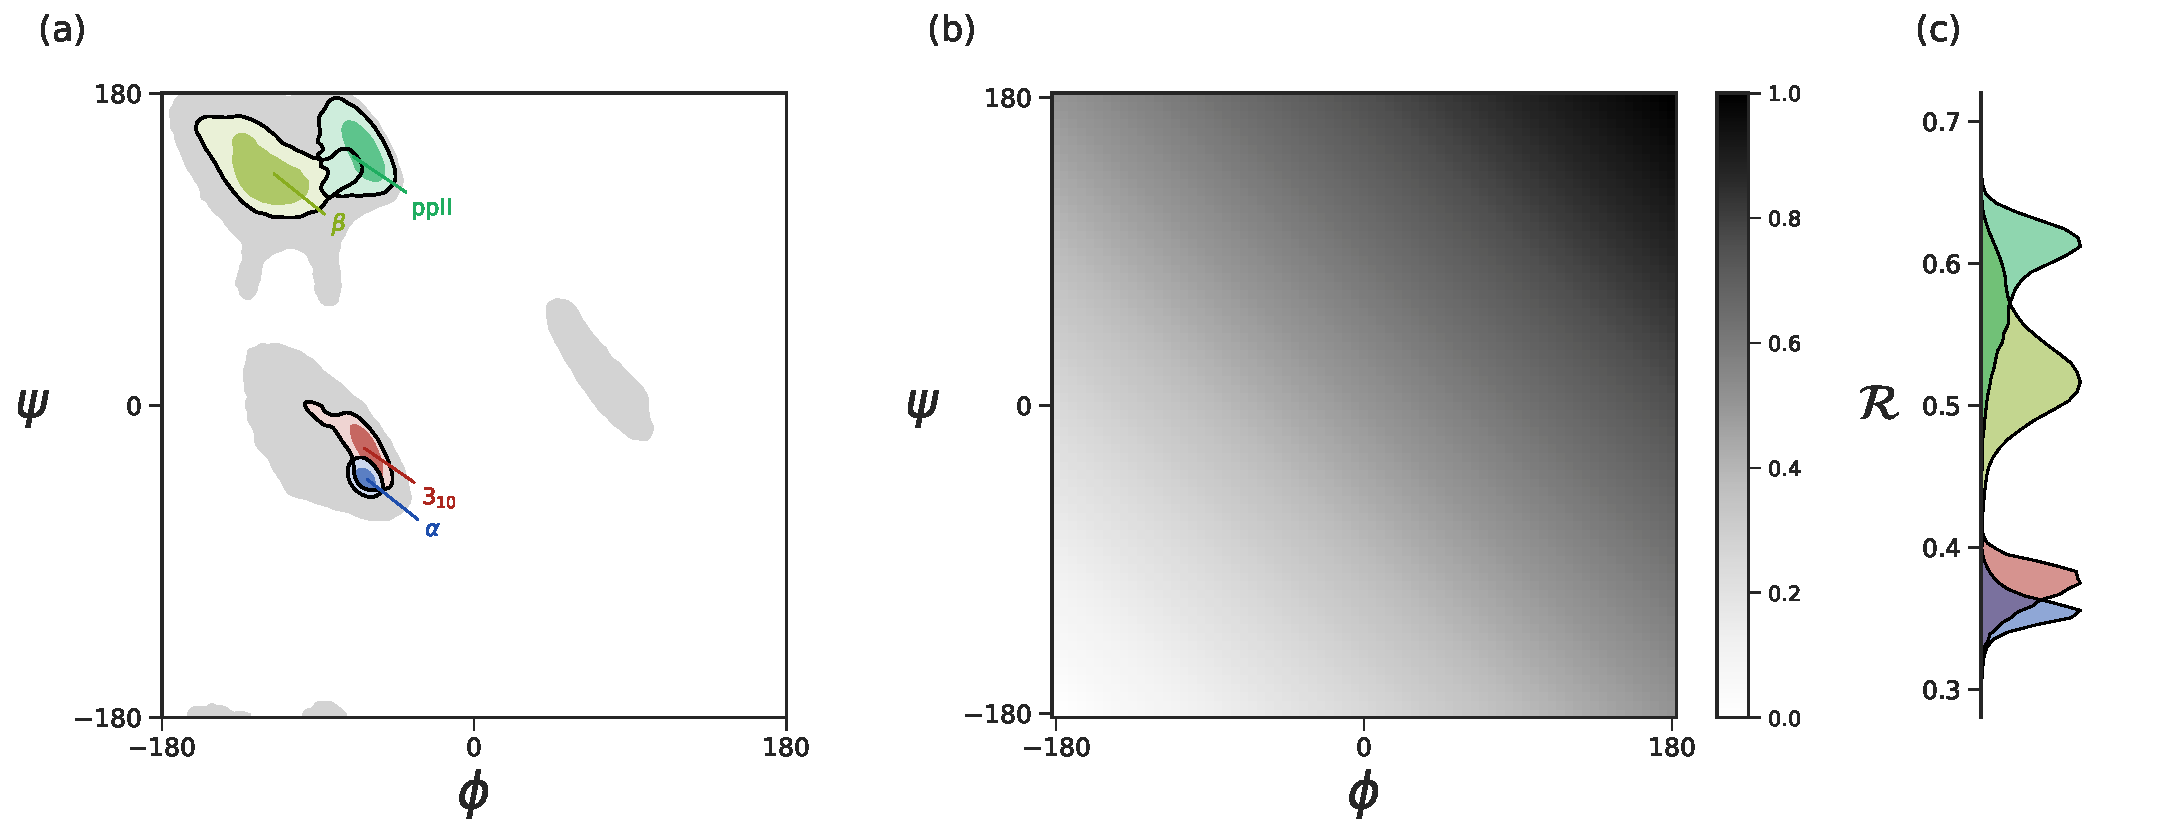
\includegraphics[width=0.9\linewidth]{backmap_fig3.pdf}
\caption{\n{Panel (a) describes the } distribution of dominant regular secondary \n{structures. Panel (b) shows the mapping between the $(\phi,\psi)$ and \rr. In Particular, \rr increases in negative-sloping sweeps from the bottom left to the top right of the Ramachandran plot. Panel (c) describes the distribution of secondary structures in \rr space. Both} Ramachandran plots (a) and Ramachandran `lines' (\n{c}) equally resolve the secondary structure space, thereby making \rr a compact yet faithful representation of backbone structure \citep{Mannige2016}.\label{fig:ramasecondary}} 
\end{adjustwidth}
\end{figure}

\section*{Introducing the \textit{simplified} Ramachandran number ($\mathcal{R}$)}

%Before expanding on the utility of the Ramachandran number, this section will present the Ramachandran number, after which a much simpler (and more accurate) version of the Ramachandran number will be described.
The Ramachandran number is both an idea and an equation. Conceptually, 
the Ramachandran number ($\mathcal{R}$) is any closed form that 
collapses the dihedral angles $\phi$ and $\psi$ into one structurally 
meaningful number \citep{Mannige2016}. \cite{Mannige2016} presented a 
version of the Ramachandran number (shown in the appendix as \Eqn{rama_old}) that was complicated in closed form, \n{thereby} reducing its utility. Here, a simpler and \n{more} accurate version of the Ramachandran number is introduced. \n{The appendix} shows how this simplified form was derived from the original closed form (\Eqns{rama_old}).

%Assuming the bounds $\phi,\psi \in [-180^\circ,180^\circ)$, and the range $\lambda$ equals $360^\circ$, the {\it simplified} 

Given arbitrary limits of $\phi \in [\phi_{\rm min},\phi_{\rm max})$ and $\psi \in [\psi_{\rm min},\psi_{\rm max})$, where the minimum and maximum values differ by $360^\circ$, the most general and accurate equation for the Ramachandran number is
\begin{equation}
{\mathcal{R}}(\phi,\psi) \equiv  \frac{\phi+\psi-(\phi_{\rm min}+\psi_{\rm min})}{(\phi_{\rm max}+\psi_{\rm max})-(\phi_{\rm min}+\psi_{\rm min})}.
\label{ramaGeneral}
\end{equation}

For consistency, we maintain throughout this paper that $\phi_{\rm min} = \psi_{\rm min} = -180^\circ$ or $-\uppi$ radians, which makes 
\begin{equation}
\mathcal{R}(\phi,\psi) = \frac{\phi+\psi+2\uppi}{4\uppi}.\label{eqn:rama}
\end{equation}

\begin{figure}[t!]
\begin{adjustwidth}{-1in}{0in} % Comment out/remove adjustwidth environment if table fits in text column.
\centering
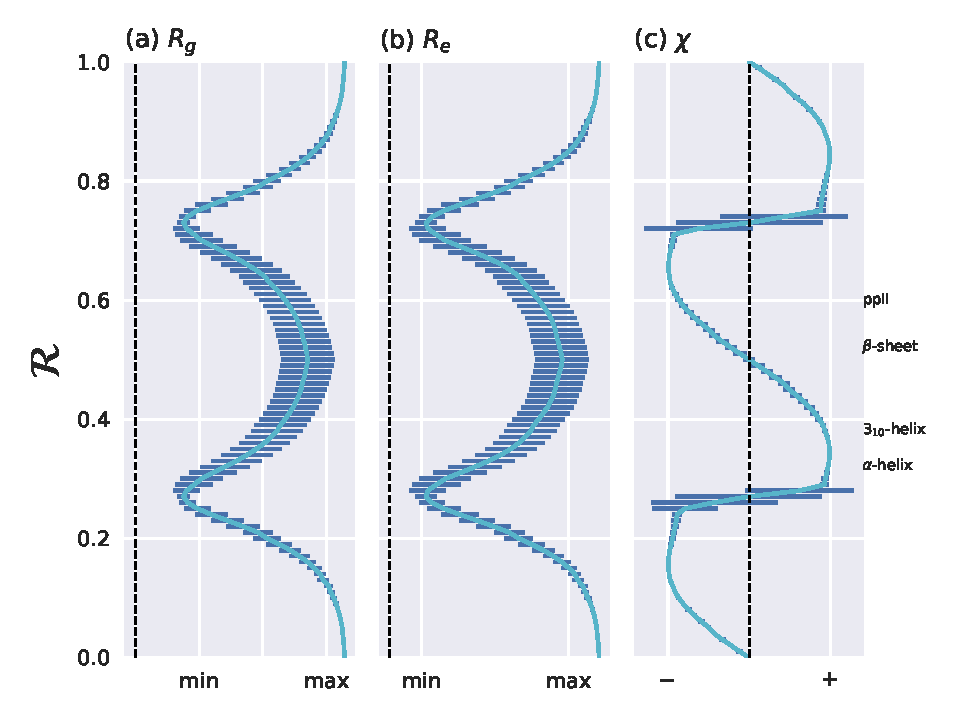
\includegraphics[width=0.6\linewidth]{backmap_fig4.pdf}
\caption{The Ramachandran number \rr displays smooth relationships with respect to radius of gyration ($R_g$; a), end-to-end distance ($R_e$; b) and chirality ($\chi$; c), as calculated within \cite{Mannige2017}. Light blue lines are average trends, dark blue horizontal lines are error bars. Average positions of dominant secondary structures are shown to the right. These trends explain why \rr is a useful and compact structural measure. Structural measures $R_g$, $R_e$\n{, and $\chi$} were obtained by computationally generating polyglycine peptides of length 10 for all possible $\phi$ and $\psi \in [-180,-175,\ldots,175,180]$. This was done using the Python library \href{https://github.com/mtien/PeptideBuilder}{PeptideBuilder} \citep{Tien2013}. Values for $R_g$, $R_e$\n{, and $\chi$} were obtained for each peptide and binned with respect to its {$\mathcal{R}(\phi,\psi)$} (each bin represents a region in \rr space that is 0.01 \rr in width). Given that actual values for $R_g$ and $R_e$ mean little (since one rarely deals with polyglycines of length 10), actual values are omitted. \n{$\chi$ ranges from -1 to +1.} \label{fig:r_smooth}} 
\end{adjustwidth}
\end{figure}


%Section~\ref{sec:simplifyR} delineates how this equation can be derived from the original closed form described in \cite{Mannige2016}.

As evident in \Fig{fig:ramasecondary}, the distributions within the Ramachandran plot are faithfully reflected in corresponding distributions within Ramachandran number space. This paper shows how the Ramachandran number is both compact enough and informative enough to generate immediately useful graphs (multi-angle pictures or MAPs) of a dynamic protein backbone.

\section*{Reason to use the Ramachandran Number}

\subsection*{Ramachandran numbers are structurally meaningful}
In addition to resolving positions of secondary structures (\Fig{fig:ramasecondary}), \rr \n{relates} well to structural measures such as radius of gyration ($R_g$), end-to-end distance ($R_e$) and chirality ($\chi$). These relationships are shown in \Fig{fig:r_smooth}. 
\n{Note that chirality comes in many forms, e.g., one could be talking about different stereo-isomers, such as L vs D amino acids, or one could be concerned with left-twisting versus right-twisting backbones, i.e., handedness \cite{Mannige2017}. This report will primarily be focused on chirality in context of backbone twist/handedness.}

\n{The trends in \Fig{fig:r_smooth} show that as one progresses from low to high \rr, various structural properties also progress smoothly. Additionally, backbones that display similar \rr also show little variation in structural properties, as evidenced by the small standard deviation bars. It is also important to note that the standard deviations shown in \Fig{fig:r_smooth} were calculated by first populating every possible region of $(\phi,\psi)$-space. However, in reality, most regions of $(\phi,\psi)$-space are unoccupied due to steric/electrostatic constraints, which means that these error bars are likely to be even smaller than depicted. Finally, the \rr number is calculated by taking `sweeps' of the  $(\phi,\psi)$-space in lines that are parallel to the negatively-sloping diagonal. Interestingly, such `sweeps' encounter only one major (dense) region within $(\phi,\psi)$-space (e.g., $\mathcal{R}$'s in the general vicinity of 0.34 represent structures that resemble $\upalpha$ helices. This means that \rr can also be used to assess the types of secondary structure present in a protein conformation.}

\begin{figure}[t!]
\centering
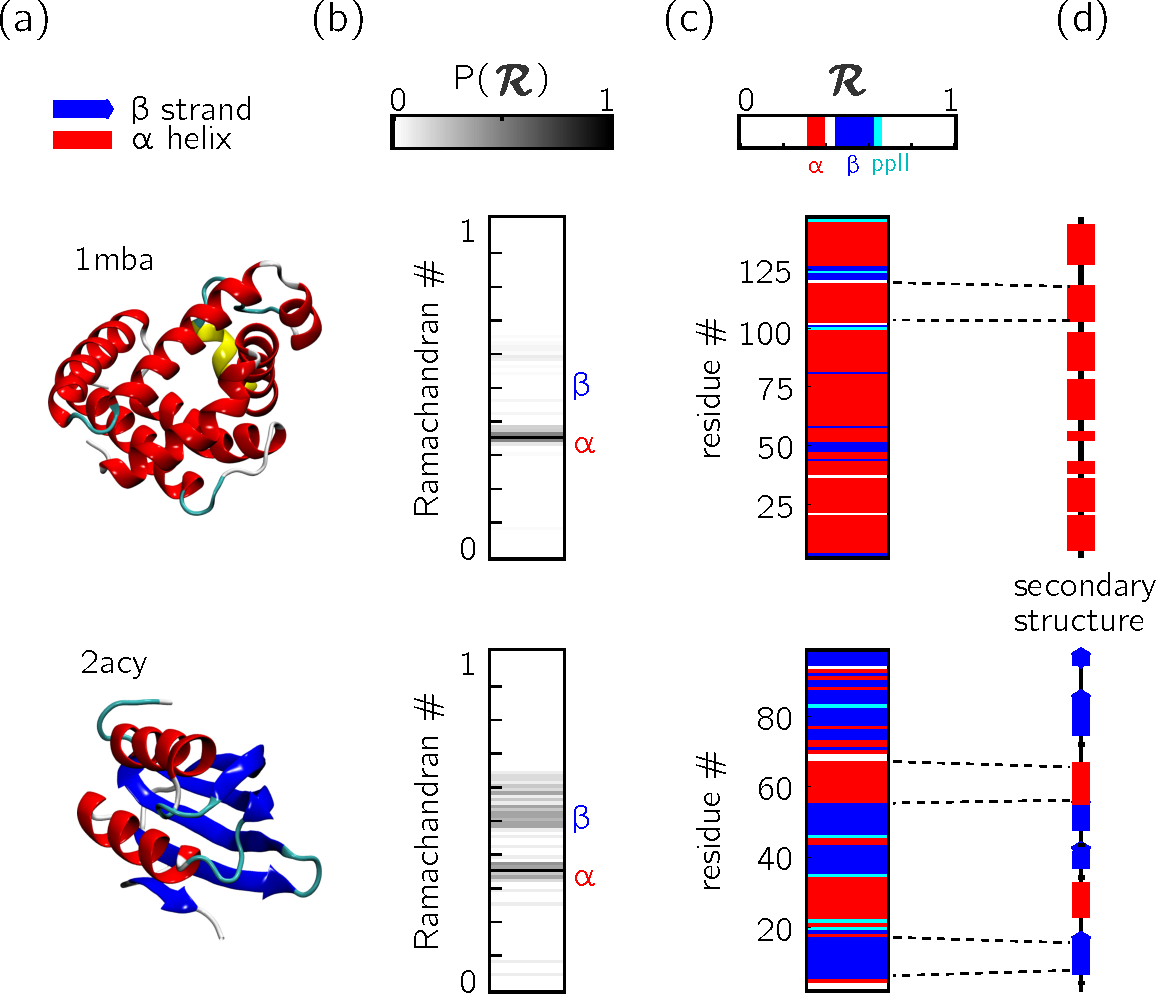
\includegraphics[width=0.65\linewidth]{backmap_fig5.pdf}
\caption{\textbf{Two types of $\mathcal{R}$-codes.} Digesting protein structures (a) using $\mathcal{R}$ numbers either as histograms (b) or per-residue codes (c) allow for compact representations of salient structural features. For example, a single glance at the histograms indicate that protein \href{https://www.rcsb.org/structure/1MBA}{1mba} is likely all $\upalpha$-helical, while \href{https://www.rcsb.org/structure/2ACY}{2acy} is likely a mix of $\upalpha$-helices and $\upbeta$-sheets. Additionally, residue-specific codes (c) not only indicate secondary structure content, but also exact \n{secondary} structure stretches (compare to d), which gives a more complete picture of how the protein is linearly arranged. \label{fig:simple_stacks}} 
\end{figure}

%\subsection*{Ramachandran numbers are more compact than one might realize} An important aspect of the Ramachandran number ($\mathcal{R}$) lies in its compactness compared to the traditional Ramachandran pair ($\phi,\psi$). Say we have an $N$-residue peptide. Then, switching from ($\phi,\psi$) to $\mathcal{R}$ \textit{appears} to only reduce the number of variables from $2N$ to $N$, and \n{hence} by half. However, ($\phi,\psi$) values are {\it coupled}, i.e., for any $N$-length peptide, any ordering of $[\phi_1,\phi_2,\ldots,\phi_N,\psi_1,\psi_2,\ldots,\psi_N]$ can not describe the structure, it is only \textit{pairs} -- $[(\phi_1,\psi_1),(\phi_2,\psi_2),\ldots,(\phi_N,\psi_N)]$ -- that can. Therefore, we must think of switching from ($\phi,\psi$)-space to $\mathcal{R}$-space as a switch in structure space per residue from $N$ two-tuples $(\phi_i,\psi_i)$ that reside in $\phi\times\psi$ space to $N$ single-dimensional numbers ($\mathcal{R}_i$).

%The value of this conversion is that the structure of a protein can be described in various one-dimensional arrays (per-structure ``Ramachandran codes'' or ``$\mathcal{R}$-codes''), which, when arranged vertically/columnarly, describe easy to digest/interpret structural patterns. See, e.g., \Fig{fig:simple_stacks}. 

\subsection*{Ramachandran codes are stackable}

\n{An important aspect of the Ramachandran number ($\mathcal{R}$) lies in its compactness compared to the traditional Ramachandran pair ($\phi,\psi$). The value of the conversion from $(\phi,\psi)$-space to \rr-space is that the structure of a protein can be described in various one-dimensional arrays (per-structure ``Ramachandran codes'' or ``$\mathcal{R}$-codes'' or multi-angle maps); see, e.g., \Fig{fig:simple_stacks}.} 

In addition to assuming a small form factor, $\mathcal{R}$-codes may then be \textit{stacked} side-by-side for visual and computational analysis. There lies its true power.


\begin{figure}[t!]
\centering
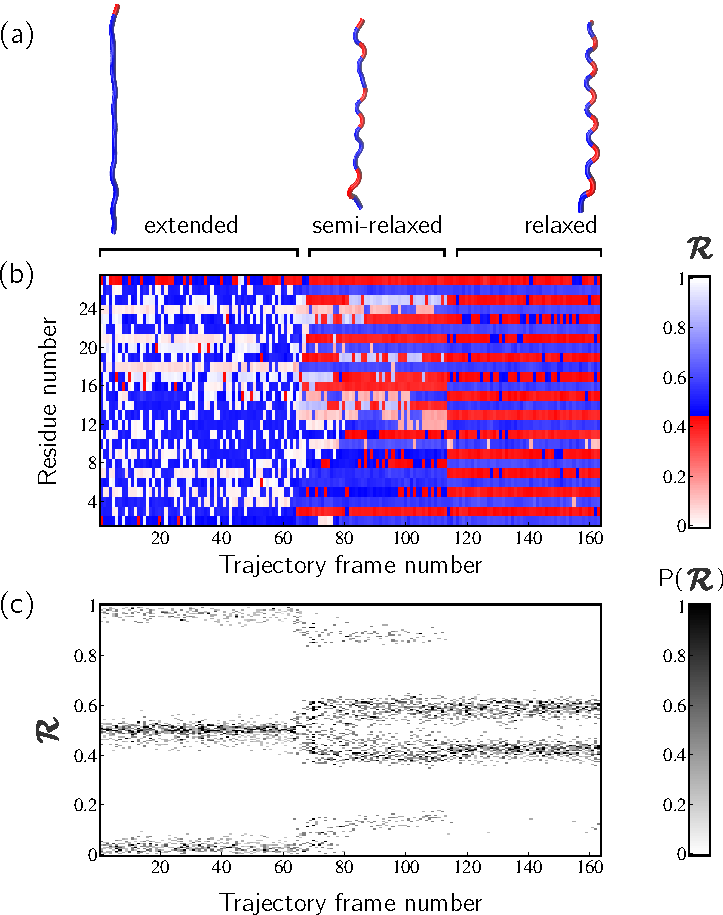
\includegraphics[width=0.65\linewidth]{backmap_fig6.pdf}
\caption{\textbf{Stacked $\mathcal{R}$-codes provide useful information at a glance.} \n{Each panel represents a molecular dynamics simulation of a peptoid nanosheet \citep{Mannige2016}, where  each peptoid backbone was held (energetically restrained) in extended state in the beginning, upon which each backbone was allowed to relax by lifting the restrains. Panel (a) displays representative structures from each stage of the simulation. Panel (b) represents how the per-resude structure of the peptide evolved over `time' (the progression of time is represented as increasing frame number). Panel (c) represents how the general distribution of backbone conformations in the peptoid (as evident by the \rr histogram) evolves over time.}\label{fig:complex_stacks}} 
\end{figure}

For example, the one-$\mathcal{R}$-to-one-residue mapping means that the entire residue-by-residue structure of a protein can be shown using a string of $\mathcal{R}_i$s (which would show regions of secondary structure and disorder, for starters). Additionally, an entire protein's backbone makeup can be shown as a histogram in $\mathcal{R}$-space (which may reveal a protein's topology). The power of this format lies not only in the capacity to distill complex structure into compact spaces, but in its capacity to display {\it many} complex structures in this format, side-by-side (stacking).

\begin{figure*}
\begin{adjustwidth}{-1in}{0in} % Comment out/remove adjustwidth environment if table fits in text column.
\centering
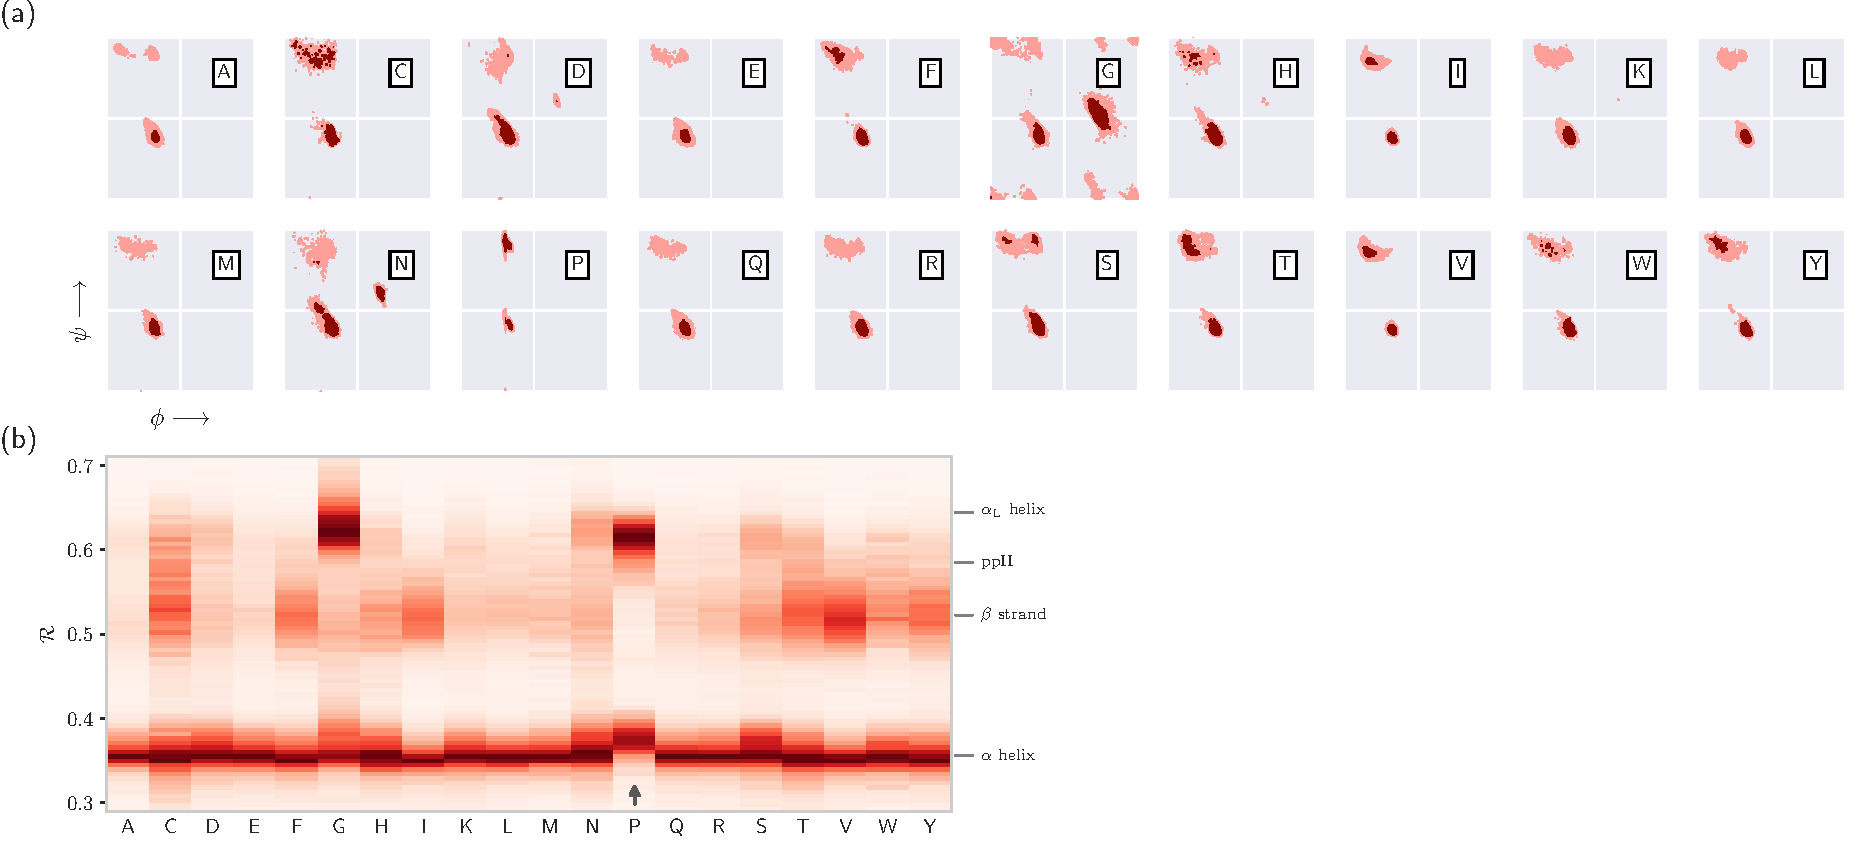
\includegraphics[width=1.00\linewidth]{backmap_fig7.pdf}
\caption{\textbf{\n{Combining Ramachandran plots for all amino acids into one graph.}}  
Panel (a) shows the per-amino acid backbone behavior of an average protein found in the protein databank (PDB). While these plots are useful, it is difficult to compare such plots. For example, it is hard to pick out the change in the $\upalpha$-helial region of the proline plot (P). However, when we convert Ramachandran plots to Rama\n{chandran} \textit{lines} [by converting $(\phi_i,\psi_i)\to\mathcal{R}_i$], we are able to conveniently ``stack'' Ramachandran lines calculated for each residue. Then, even visually, it is obvious that proline does not occupy the canonical $\upalpha$-helix region, which is not evident to an untrained eye in (a).\label{fig:peraa}}
~\vfill~
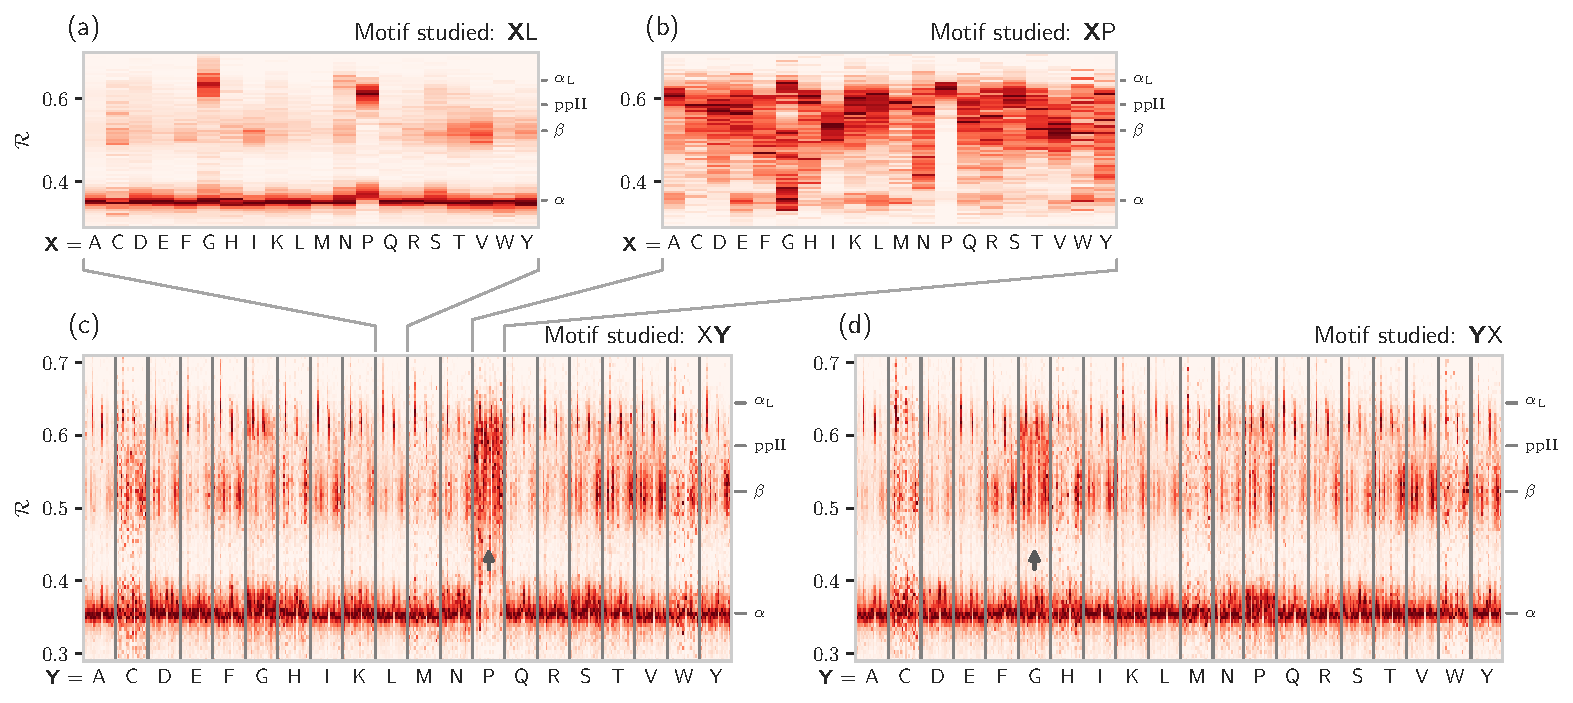
\includegraphics[width=1.00\linewidth]{backmap_fig8.pdf}
\caption{\textbf{\n{How residue neighbors modifies structure.}} Similar to \Fig{fig:peraa}b, Panel (a) represents the behavior of an amino acid `X' situated {\it before} a leucine (XL; assuming that we are reading a sequence from the N terminal to the C terminal). Panel (b) similarly represents the behavior of specific amino acids situated before a proline (XP). While residues preceeding a leucine behave similarly to their average behavior (\Fig{fig:peraa}a), most residues preceeding prolines appear to be enriched in structures that change `direction' or backbone chirality (this is evident by many amino acids switching from \rr$<0.5$ to \rr$>0.5$). 
Panel\n{s} (c) \n{and (d) show} the behavior of individual amino acids when situated before \n{and after} each of the 20 amino acids\n{, respectively}. 
%\n{Panel (d) shows the behavior of individual amino acids after each of the 20 amino acids.}
\n{Panels (c) and (d)} show a major benefit of side-by-side Ramachandran line ``stacking'': general trends become much more obvious. For example, it is evident that prolines dramatically modify the structure of an amino acid preceeding it (compared to average behavior of amino acids in \Fig{fig:peraa}b)\n{, while residues following glycines also have a higher prevalence of $\mathcal{R} > 0.5$ conformations (both trends are indicated by small arrows)}. 
Such trends, while previously discovered \n{(see text)}, would not be accessible when na{\"i}vely considering Ramachandran plots because one would require 400 ($20\times 20$) distinct Ramachandran plots to compare. \n{Note that the statistics for each \rr-line in (c) and (d) are dependent on the joint prevalence of the residues being considered. For this reason, some \rr-lines (e.g., those associated with cysteines) look more rough or `dotty' than others.}.%Panel (d) facetiously represents 800 tiny Ramachandran plots, emphasizing how hard it would be to make such comparisons using Ramachandran plots.
\label{fig:motifs}}
\end{adjustwidth}
\end{figure*}

Peptoid nanosheets \citep{Mannige2015} will be used here as an example of how multiple structures, in the form of \rr-codes, may be stacked to provide immediately useful pictograms. \n{Peptoids are stereo-isomers of peptides, where the sidechain is attached to the backbone nitrogen 
rather than the $\upalpha$ carbon atom. Since both peptoids and peptides share identical backbone connectivity, the analysis described below could be applied to both peptides and peptoids.}

Peptoid nanosheets are a recently discovered peptide-mimic that, in one molecular dynamics simulation \citep{Mannige2015}, were shown to display a novel secondary structure. In the reported model \citep{Mannige2015}, each peptoid within the nanosheet displays backbone conformations that alternate in chirality, causing the backbone to look like a meandering snake that nonetheless maintains an overall linear direction. This secondary structure was discovered by first setting up a nanosheet where all peptoid backbones were restrained to be fully extended (\Fig{fig:complex_stacks}a, left), after which the restraints were energetically softened (a, middle) and completely \n{released} (a, right). As evident in \Fig{fig:complex_stacks}b and \Fig{fig:complex_stacks}c, the two types of \rr-code stacks display salient information at first glance: 1) \Fig{fig:complex_stacks}b shows that the extended backbone first undergoes some rearrangement with softer restraints, and then becomes much more binary in arrangement as we look down the backbone (excepting the low-order region in the middle, unshown in \Fig{fig:complex_stacks}a); and 2) \Fig{fig:complex_stacks}c shows that lifting restraints on the backbone causes a dramatic change in backbone topology, namely a birth of a bimodal distribution evident in the two parallel horizontal bands.

By utilizing \rr, maps such as those in \Fig{fig:complex_stacks} provide information about every $\phi$ and $\psi$ within the backbone. As such, these maps are dubbed MAPs, for Multi Angle Pictures. A Python package called \pname created \Fig{fig:complex_stacks}a and b, which is provided as a GitHub repository at \url{https://github.com/ranjanmannige/\gname}. \pname takes in a PDB structure file containing a single structure, or multiple structures separated by the code `MODEL'.

\subsection*{Case study: picking out subtle differences from high volume of data}

This section expands on the notion that \rr-numbers -- due to their compactness/stackability -- can be used to pick out backbone structural trends that would be hard to decipher using any other metric. For example, it is well known that prolines (P) display unusual backbone behavior: in particular, proline backbones occupy structures that are close to but distinct from $\upalpha$-helical regions. Due to the two-dimensionality of Ramachandran plots (\Fig{fig:peraa}a), such distinctions are hard to visually pick out from Ramachandran plots. However, stacking per-amino-acid \rr-codes side by side make such differences patent (\Fig{fig:peraa}b; see arrow).

It is also known that amino acids preceeding prolines display unusual shift in backbone twist/chirality. For example, \Fig{fig:motifs}c shows that amino acids appearing before prolines behave differently than they would otherwise \n{(see the upward-facing arrow)}. \n{Additionally, amino acids {\em following} glycines also appear to have their structures modified (\Fig{fig:motifs}d; upward arrow).} 
\n{Note that these results are not new, and it has already been confirmed that, e.g., nearest neighbors affect the conformational behavior of an animno acid as witnessed within Ramachandran plots \citep{Ting2010}, and proline changes the backbone conformation of the preceeding residue \citep{Gunasekaran1998,Ho2005}. %they were reported more than 30 years after the first structures were published; they would have been relatively easy to find if \rr-codes were to be used regularly. 
However, \Figs{fig:peraa} and \ref{fig:motifs} indicate that such information can be more concisely shown/identified when structures are stacked side-by-side in the form of $\mathcal{R}$-codes.} Such subtle changes are often witnessed when protein backbones transition from one state to another.

\section*{Using the \pname Python Module}

\subsection*{Installation}
\pname may either be installed locally by downloading the \href{https://github.com/ranjanmannige/backmap}{GitHub repository}, or installed directly by running the following line in the command prompt (assuming that \code{pip} exists): \code{> pip install backmap}

\subsection*{Usage}
The module can either be imported and used within existing scripts, or used as a standalone package using the command `python -m backmap'. First the in-script usage will be discussed.

\subsection*{In-script usage I: first simple test}
The simplest test would be to generate Ramachandran numbers from $(\phi,\psi)$ pairs:
\begin{python}
# Import module
import backmap 
# Convert (phi, psi) to R
print backmap.R(phi=0,phi=0) # Expected output: 0.5
print backmap.R( -180, -180) # Expected output: 0.0
print backmap.R(  180,  180) # Expected output: 1.0 (equivalent in meaning to 0)
\end{python}

\subsection*{In-script usage II: basic usage for creating Multi-Angle Pictures (MAPs)}
The following code shows how Multi-Angle Pictures (MAPs) of protein backbones can be generated:
\begin{enumerate}
\item {\bf Select and read a protein PDB structure}\\
Each trajectory frame must be a set of legitimate protein databank "ATOM" records separated by "MODEL" keywords (distinct models show up as distinct frames on the x-axis or abscissa).
\begin{python}[firstnumber=1]
import backmap 
pdbfn = './pdbs/nanosheet_birth_U7.pdb' # Set pdb name 
data = backmap.read_pdb(pdbfn) # READ PDB in the form of a matrix with columns
\end{python}
Here, `\code{data}' is a 2d array with four columns [`\code{model}', `\code{chain}', `\code{resid}',`\code{R}']. 
The first row of `\code{data}' is the header (i.e., the name of the column, e.g., `\code{model}'), 
with values that follow.
\item {\bf Select color scheme (color map)}\\
In addition to custom colormaps listed in the next section, one can also use \n{traditionally} available colormaps at 
\href{http://matplotlib.org/examples/color/colormaps_reference.htm}{matplotlib.org} (e.g., `\code{Reds}' or `\code{Reds\_r}').
\ContinueLineNumber
\begin{python}
# setting the name of the colormap
cmap = "SecondaryStructure"
\end{python}
\item {\bf Draw per-chain MAPs}
\ContinueLineNumber
\begin{python}
# Grouping by chain
grouped_data = backmap.group_by(data,group_by='chain',
                            columns_to_return=['model','resid','R'])
for chain in grouped_data.keys(): # Going through each chain
	# Getting the X,Y,Z values for each entry
	models, residues, Rs = grouped_data[chain]
	# Finally, creating (but not showing) the graph 
	backmap.draw_xyz(X = models  ,      Y = residues  ,     Z = Rs
	           ,xlabel ='Frame #', ylabel ="Residue #",zlabel ='$\mathcal{R}$'
	             ,cmap = cmap    ,  title = "Chain: '"+chain+"'"
	             ,vmin=0,vmax=1)
	# Now, we display the graph:
	plt.show() # ... one can also use plt.savefig() to save to file
\end{python}
Running the module as a standalone script would produce all these graphs automatically.
`\code{plt.show()}' would result in the following image being rendered:\\
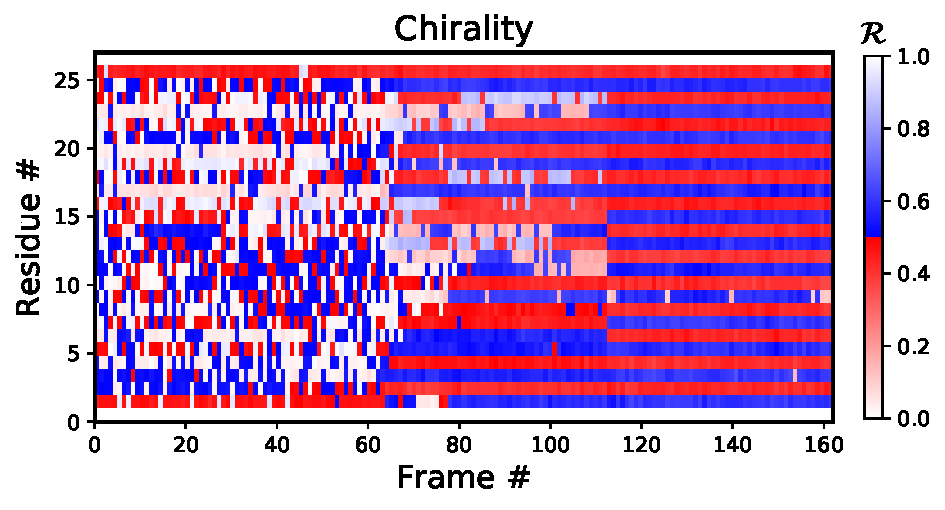
\includegraphics[width=0.5\linewidth]{backmap_figA.pdf}

Additionally, by changing how one assigns values to `X' and `Y', 
one can easily construct and draw other types of graphs such as time-resolved histograms, 
\n{per-residue fluctuations when compared to the first ($D_{1}$) and previous structure ($D_{-1}$) within the trajectory}, etc. 
\end{enumerate}

\subsection*{In-script usage III: Creating custom graphs}
Other types of \n{graphs} can be easily created by modifying part three of the code above. 
For example, the following code creates histograms of R, one for each model (starting from line 9 above).
\begin{python}[firstnumber=9]
	for chain in grouped_data.keys():
		models, residues, Rs = grouped_data[chain]
		
		'Begin custom code'
		X = []; Y=[]; Z=[]; # Will set X=model, Y=R, Z=P(R)
		# Bundling the three lists into one 2d array
		new_data =  np.array(zip(models,residues,Rs))
		# Getting all R values, model by model
		for m in sorted(set(new_data[:,0])): # column 0 is the model column
			# Getting all Rs for that model #
			current_rs = new_data[np.where(new_data[:,0]==m)][:,2] # column 2 contains R
			# Getting the histogram
			a,b = np.histogram(current_rs,bins=np.arange(0,1.01,0.01))
			max_count = float(np.max(a))
			for i in range(len(a)):
				X.append(m); Y.append((b[i]+b[i+1])/2.0); Z.append(a[i]/float(np.sum(a)));
		'End custom code'
		
		# Finally, creating (but not showing) the graph 
		draw_xyz(X = X       ,      Y = Y  ,                Z = Z
		   ,xlabel ='Frame #', ylabel ="$\mathcal{R}$",zlabel ="$P'(\mathcal{R})$"
			 ,cmap = 'Greys', ylim=[0,1])
		plt.yticks(np.arange(0,1.00001,0.2))
		# Now, we display the graph:
		plt.show() # ... one can also use plt.savefig() to save to file
\end{python}
The code above results in the following graph:\\
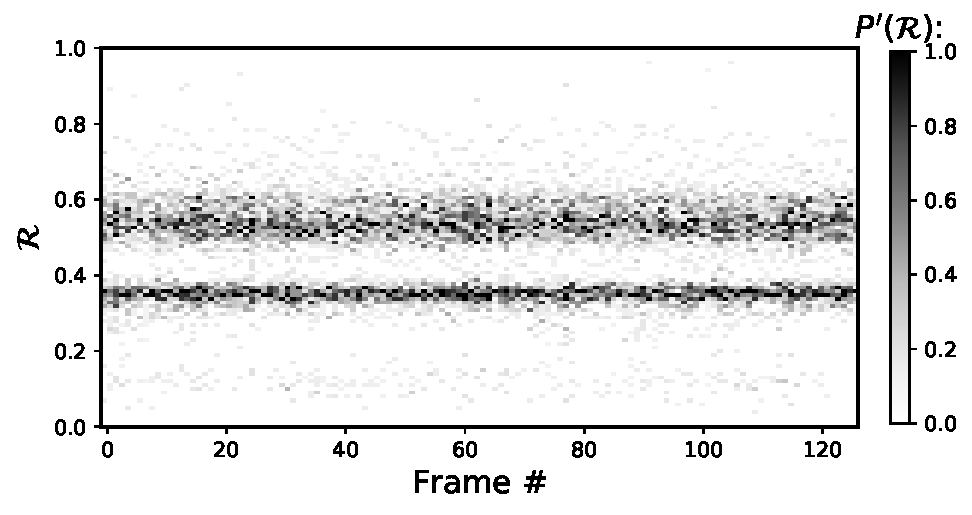
\includegraphics[width=0.5\linewidth]{backmap_figB.pdf}

\subsection*{In-script usage IV: Available color schemes (CMAPs)}
Aside from the general color maps (cmaps) that exist in matplotlib (e.g., `Greys', `Reds', or, god forbid, `jet'), 
\pname provides two new colormaps: `\code{Chirality}' (key: $+$-twists -- red; $-$ve twists: blue), and `\code{SecondaryStructure}' (key: {\it potential} helices -- red; sheets -- blue; ppII helices -- cyan). right twisting backbones are shown in red; left twisting backbones are shown in blue). \Fig{fig:cmaps} shows how a single protein ensemble
may be described using these schematics. As illustrated in \Fig{fig:cmaps}b, cmaps available within the standard matplotlib package do not distinguish between major secondary structures well, while those provided by \pname do. In case it is known that the protein backbone accesses non-traditional regions of the Ramachandran plot, a four-color schematic will be needed (see below for more discussions).

\begin{figure}[h!]
\centering
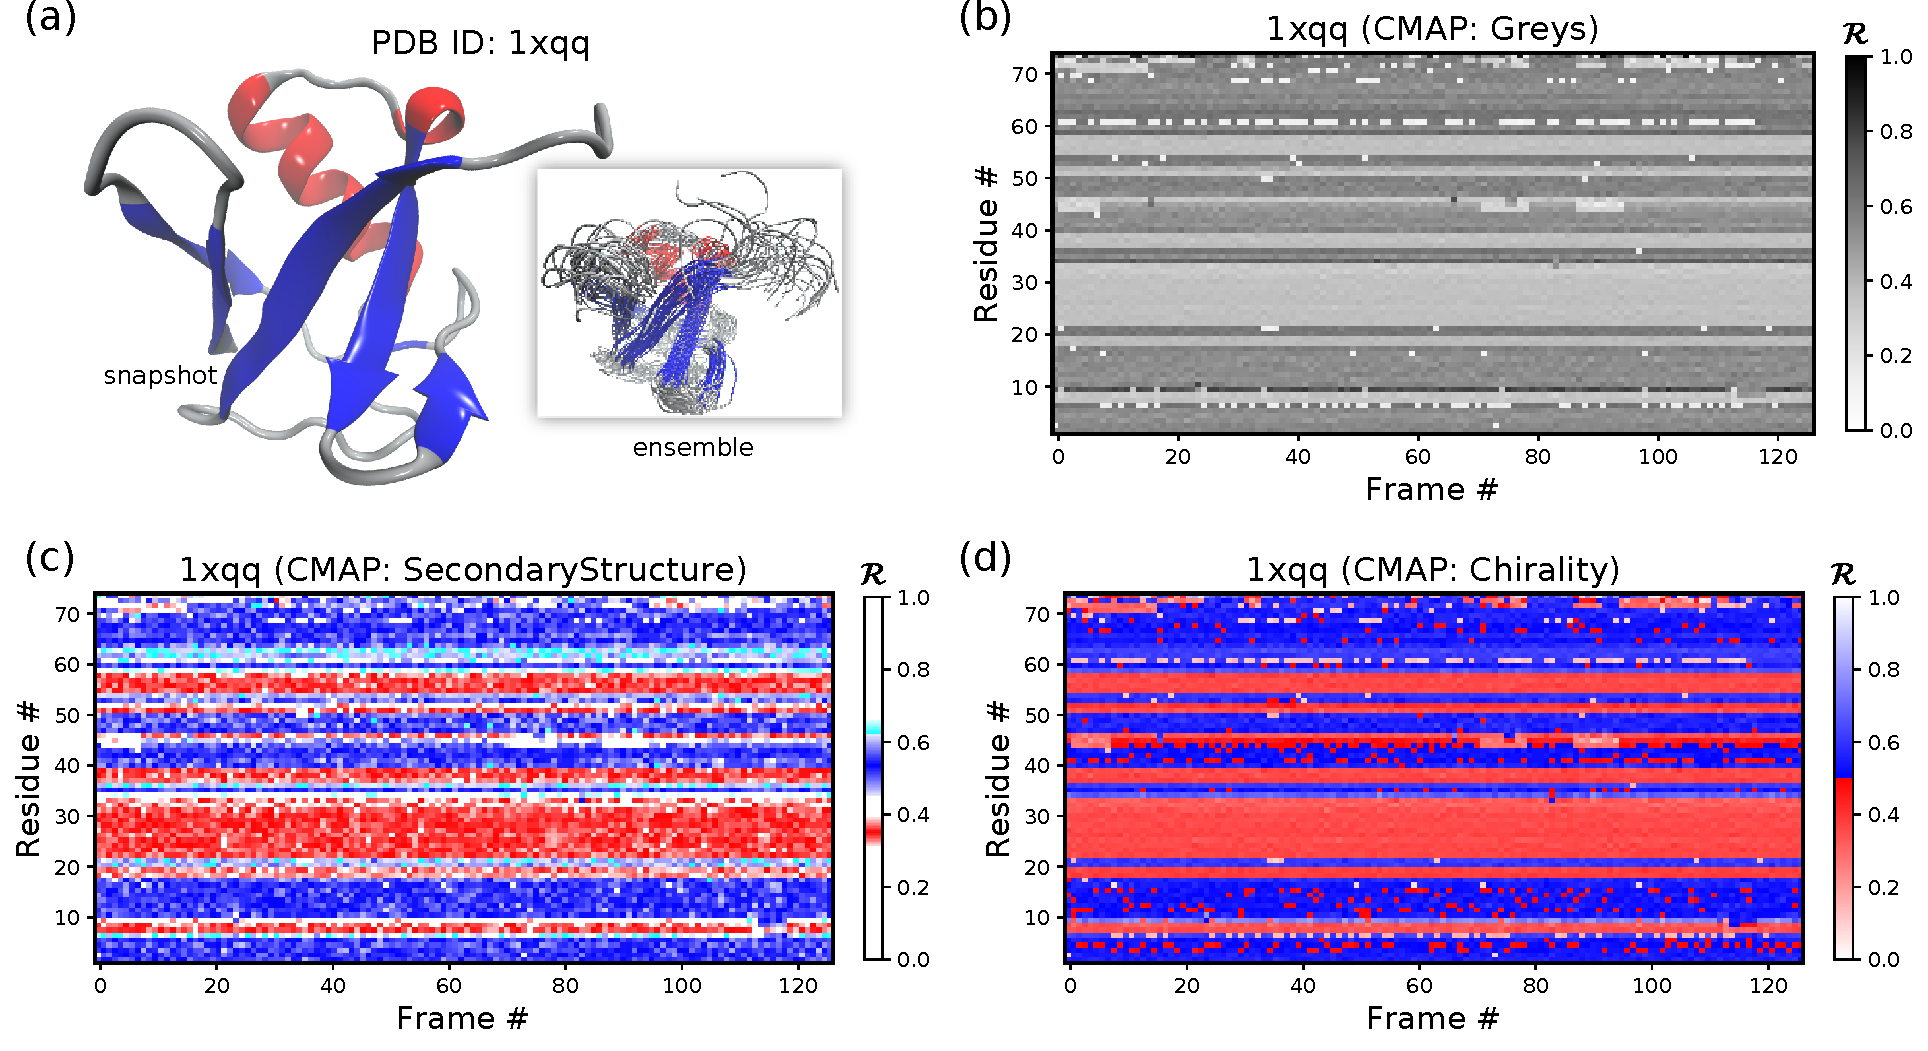
\includegraphics[width=0.9\linewidth]{backmap_fig9.pdf}
\caption{A protein ensemble (a) along with some MAPs colored with different themes (b-d). Panels (c) and (d) are provided by the \pname module. In Panel (c), $\upbeta$-sheets are shown in blue and all helices are shown in red. In Panel (d), right-handed and left-handed backbone twists are shown as red and blue respectively.\label{fig:cmaps}} 
\end{figure}

\subsection*{Stand Alone Usage}

\pname can be used as a stand along package by running `> python -m backmap -pdb <pdb\_dir\_or\_file>'. The sectons below describes the expected outputs and how they may be interpreted.

\begin{figure*}[t!]
%\centering
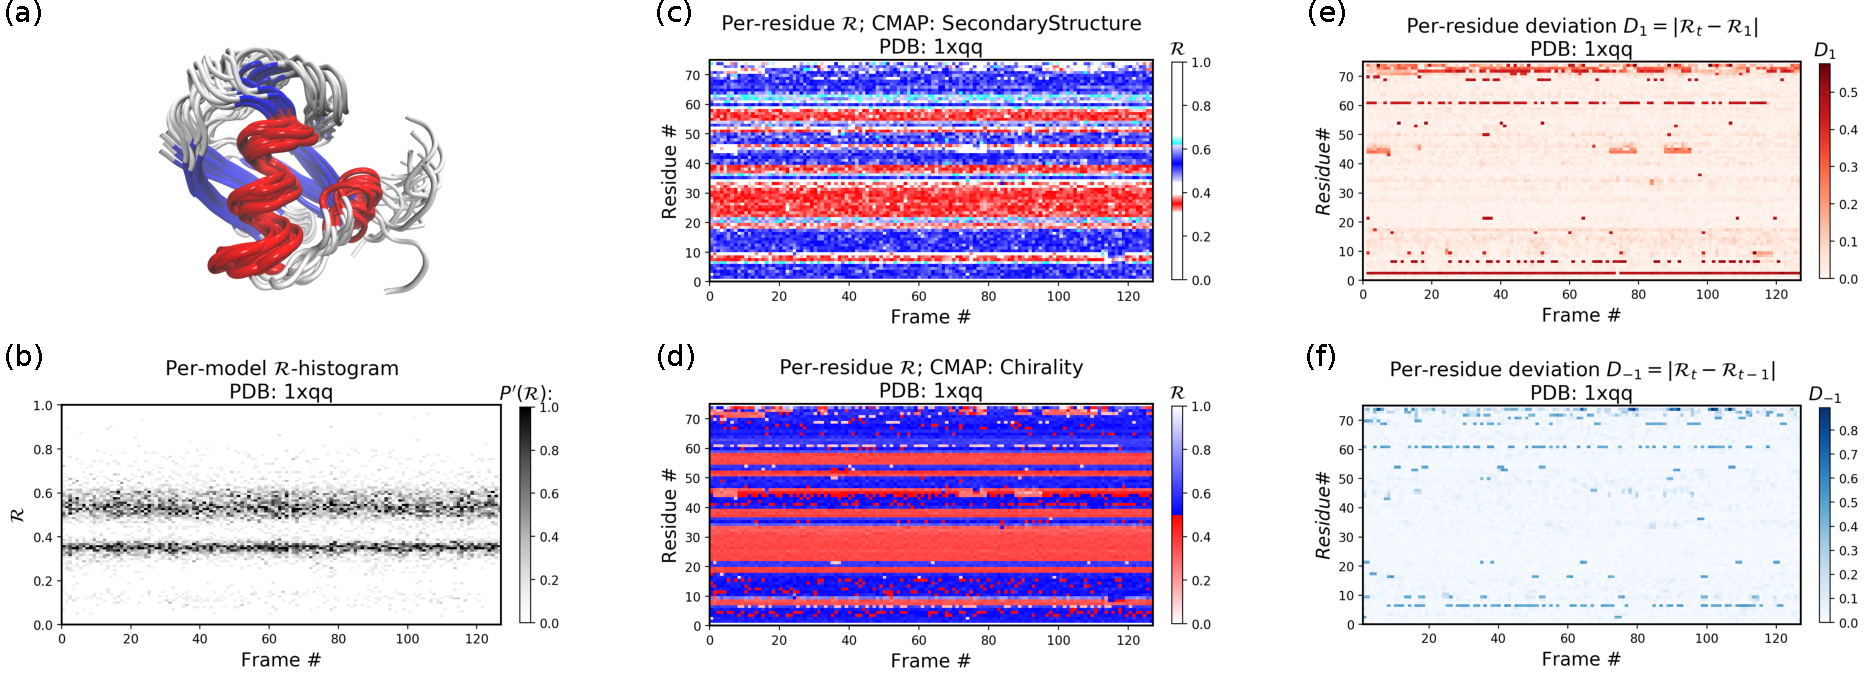
\includegraphics[width=1.0\linewidth]{backmap_fig10.pdf}
\caption{Protein \href{https://www.rcsb.org/structure/1XQQ}{1xqq} describes a stable protein. \n{Panel (a) represents the entire ensemble, Panel(b) represents a histogram distribution of \rr, Panels (c) and (d) represent two ways color per-residue \rr plots, and Panels (e) and (f) are two ways to describe backbone fluctuation over time.}\label{fig:example1}} 
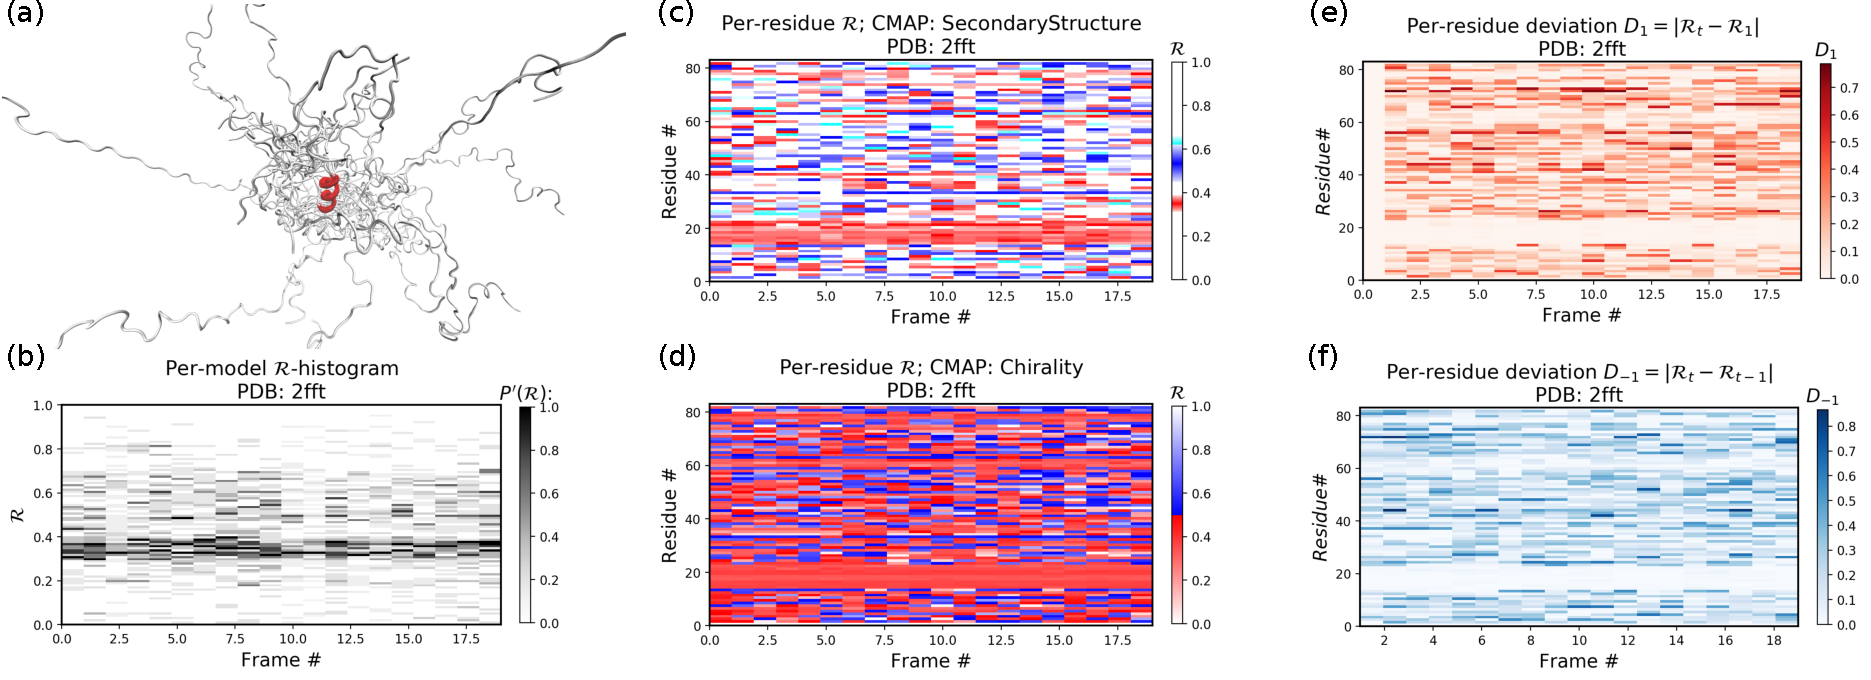
\includegraphics[width=1.0\linewidth]{backmap_fig11.pdf}
\caption{Protein \href{https://www.rcsb.org/structure/2FFT}{2fft} describes an intrinsically disordered protein, with one stable helix in red.
\n{Descriptions of each panel are identical to that of \Fig{fig:example1}.}\label{fig:example2}} 
\end{figure*}

\subsection*{Stand Alone Example I: A Stable Protein}

Panels (b) through (f) of \Fig{fig:example1} below were created by running `> python -m backmap ./tests/pdbs/1xqq.pdb' (Panel (a) was created using \href{http://www.ks.uiuc.edu/Research/vmd/}{VMD}). These graphs indicate that protein \href{https://www.rcsb.org/structure/1XQQ}{1xqq} describes a conformationally stable protein, since each residue fluctuates little in color (structure) over `time' (c,d; here and below, it is assumed that discrete models represent distinct states of the protein over `time'), show little change in the \rr histogram over time (b) and show few enduring fluctuations \n{(e,f; see Methods)}. 

In particular, each column in Panel (b) describes the histogram in Ramachandran number (R) space for a single model/timeframe. These histograms show the presence of both $\upalpha$-helices (at $\mathcal{R} \approx 0.34$) and $\upbeta$-sheets (at $\mathcal{R} \approx 0.52$). Additionally, Panels (c) and (d) describe per-residue conformational plots (colored by two different metrics or CMAPs), which show that most of the protein backbone remains relatively stable over time (e.g., few fluctuations in state or `color' are evident over frame \#). Finally, Panel (e) describes the extent towards which a single residue's state has deviated from the first frame, and Panel (f) describes the extent towards which a single residue's state has deviated from its state in the previous frame. All these graphs, show that this protein is relatively conformationally stable.

\subsection*{Stand Alone Example II: An Intrinsically Disrodered Protein}

\Fig{fig:example2} is identical to \Fig{fig:example1}, except that the panels pertain to an intrinsically disordered protein \href{https://www.rcsb.org/structure/2FFT}{2fft} whose structural ensemble describes dramatically distinct conformations. 

As compared to the conformationally stable protein above, protein \href{https://www.rcsb.org/structure/2FFT}{2fft} is much more flexible. Panel (b) shows that the states accessed per model are diverse and dramatically fluctuate over the entire range of $\mathcal{R}$ (this is especially true when compared to a stable protein, see \Fig{fig:example1}b). 

The diverse states occupied by each residue (Panels (c) and (d)) confirm the conformational variation displayed by most of the backbone (Panels (e) and (f) similarly show how most of the residues fluctuate dramatically).

Yet, interestingly, Panels (c) through (f) also show an \n{unusually} stable region -- residues 15 through 25 -- which consistently display the same conformational ($\upalpha$-helical) state at $\mathcal{R}\approx0.34$ (interpreted as the color red in Panel (c)). This trend would be hard to recognize by simply looking at the structural ensemble (Panel (a)). 

\subsection*{A signed Ramachandran number for `misbehaving' backbones}

%The Ramachandran number maps the two dimensional $(\phi,\psi)$-space into one number by ensuring that points that lie on lines parallel to the negative diagonal are most similar to eachother. I.e., 
The Ramachandran number increases in value from the bottom left of the Ramachandran plot to the top right in sweeps that are parallel to the negative sloping diagonal. As discussed in \cite{Mannige2016}, this method of mapping a two-dimensional space into one number is still structurally meaningful and descriptive because 1) most structural features of the protein backbone -- e.g. radius of gyration \citep{Mannige2016}, end-to-end distance \citep{Mannige2016}, and chirality \citep{Mannige2017} -- vary little along lines parallel to the negatively-sloping diagonal (this is indicated by relatively small standard deviations in structural metrics for similar {\rr}s; \Fig{fig:r_smooth}), and 2) most protein backbones display chiral centers and therefore predominantly appear on the top left region of the Ramachandran plot (above the dashed diagonal in \Fig{fig:signed}a-{\it(i)}).

\begin{figure*}[t!]
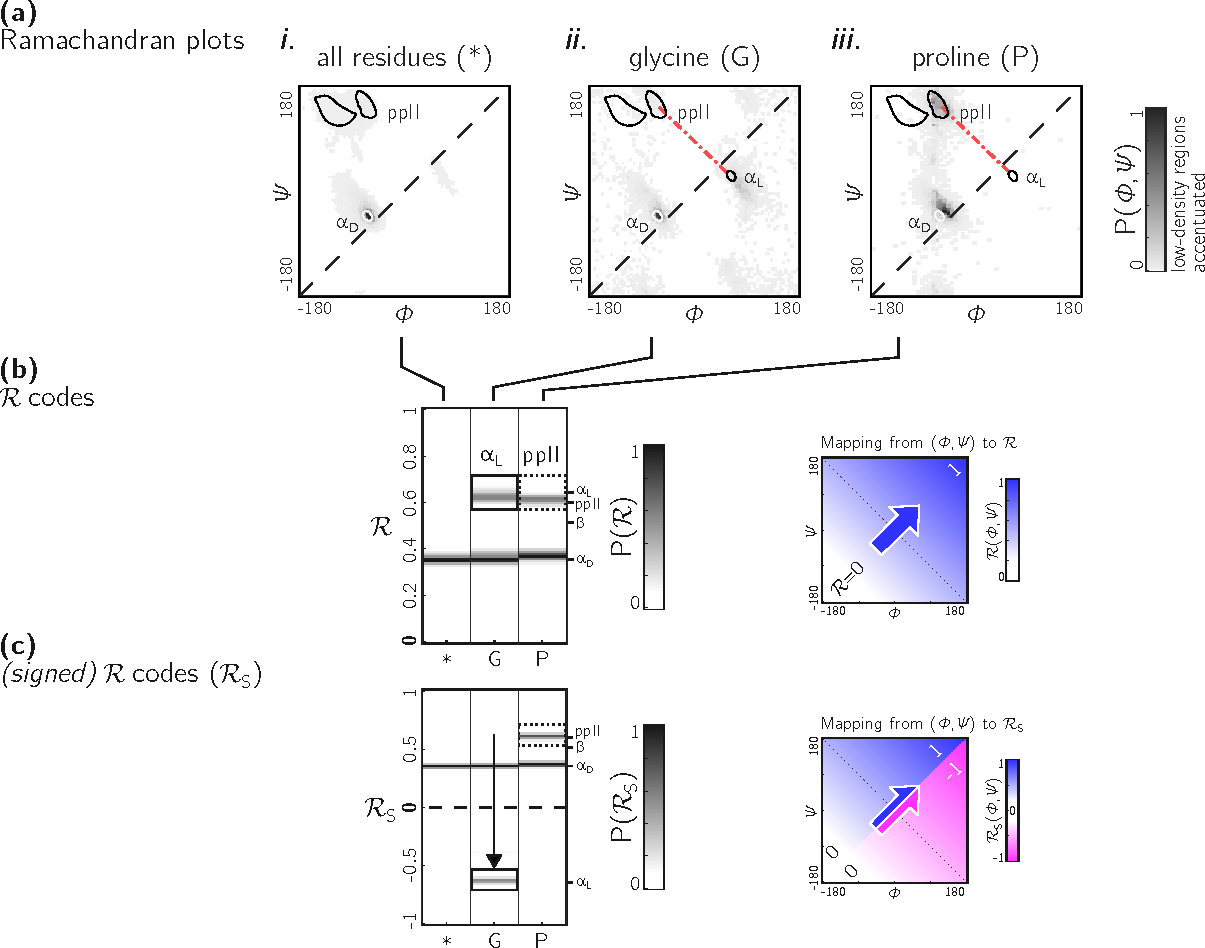
\includegraphics[width=1.0\linewidth]{backmap_fig12.pdf}
\caption{\textbf{Signed {\rr}s are required for non-chiral backbones.} While the backbones of most amino acids occupy the top of the positively sloped diagonal (dashed in b), non chiral amino acids such as Glycines (or their N-substituted variants -- peptoids) display no such preference, which causes distinct secondary structures that lie on the same `sweep' to be localized at similar regions in \rr (e.g., in b, polyproline-II and $\upalpha_\textrm{D}$ helices both localize at \rr $\approx 0.6$). However, a signed Ramachandran number ($\mathcal{R}_\textrm{S}$) solves this overlap by multiplying those \rr's derived from backbones with $\phi > \psi$ by $-1$. The resolving power of $\mathcal{R}_\textrm{S}$ is evident by the separation of polyproline-II and $\upalpha_\textrm{D}$ helices (c). The mapping of $(\phi,\psi)$ to $\mathcal{R}$ and $\mathcal{R}_\textrm{S}$ are shown to the right of each respective \rr-plot (b,c).\label{fig:signed}} 
\end{figure*}

However, not all backbones localize in only one half of the Ramachandran plot. Particularly, among biologically relevant amino acids, glycine occupies both regions of the Ramachandran plot (\Fig{fig:signed}a-{\it(ii)}; of note, the $\upalpha_\textrm{L}$ helix region becomes relatively prominent). On the other hand, prolines are known to form polyproline-II helices ($\textrm{ppII}$ in \Fig{fig:signed}a-{\it(iii)}), which falls on almost the same `sweep' as glycine rich peptides (red dot-dashed line). In situations where both prolines and glycines are abundant, the Ramachandran number (\rr) would fail to distinguish $\upalpha_\textrm{L}$ from $\textrm{ppII}$ (\Fig{fig:signed}b; regions outlined by rectangles).


To accomodate the situation where achiral backbones are expected (eg., if peptoids or polygycines are being studied), an additional Ramachandran number -- the \textit{signed} Ramachandran number $\mathcal{R}_\textrm{S}$ -- is introduced here. $\mathcal{R}_\textrm{S}$ is identical to the original number in magnitude, but which changes sign from $+$ to $-$ as you approach $\mathcal{R}$ numbers that are to the right (or below) the positively sloped diagonal. I.e., 
\begin{equation}
\mathcal{R}_\textrm{S} = 
\begin{cases}
    \mathcal{R}         &\text{, if } \psi \geq \phi  \\
    \mathcal{R}\times-1 &\text{, if } \psi   <  \phi
\end{cases}\label{eqn:signed}
\end{equation}
As an example of the utility of $\mathcal{R}_\textrm{S}$, \Fig{fig:signed}c shows that $\mathcal{R}_\textrm{S}$ easily distinguishes $\upalpha_\textrm{D}$ from $\textrm{ppII}$.

Note that the signed $\mathcal{R}_\textrm{S}$, while useful, would be important in very limited scenarios, as more than 96\% of the amino acids in the Protein Databank (PDB) occupy the upper-left region of the Ramachandran plot (with the 3\% of `rule breakers' contributed mostly by glycines).

\section*{Conclusion}

A simpler Ramachandran number is reported -- $\mathcal{R} = (\phi+\psi+2\pi)/(4\pi)$ -- which, while being a single number, provides much information. For example, as discussed in \cite{Mannige2016}, \rr values above 0.5 are left-handed \n{in twist}, while those below 0.5 are right handed, \rr values close to 0, 0.5 and 1 are extended, $\upbeta$-sheets occuppy \rr values at around 0.52, right-handed $\upalpha$-helices hover around 0.34. Given the Ramachandran number's `stackability', single graphs can hold detailed information of the progression/evolution of molecular trajectories. Indeed, \Fig{fig:motifs} shows how 400 distinct Ramachandran plots can easily be fit into one graph when using \rr. Finally, a python script/module (\pname) has been provided in an online \href{https://github.com/ranjanmannige/\gname}{GitHub repository} to promote the utility of \rr as a universal metric.

\section*{Materials}

Statistics about single amino acid conformations and secondary structures (excepting polyproline II helices) were derived from the Structural Classification of Proteins or SCOPe website [Release 2.06; \cite{Fox2014}]. This database, currently available at  \url{http://scop.berkeley.edu/downloads/pdbstyle/pdbstyle-sel-gs-bib-40-2.06.tgz}, contains 13,760 three-dimensional protein conformations (one domain per conformation) with lower than 40\% sequence identity. Secondary structure annotations were assigned using the DSSP algorithm \citep{Kabsch1983}, although the STRIDE algorithm \citep{Frishman1995} provides qualitatively identical distributions. \n{These statistics were used to produce distributions within \Fig{fig:ramaintro}a and \Fig{fig:ramasecondary}a,c.}

Given the absence of polyproline II helix (ppII) annotation in the 
present version of DSSP, statistics for polyproline II helices 
\n{(used to generate the ppII distributions in \Fig{fig:ramaintro}a and \Fig{fig:ramasecondary}a,c)} were obtained from segments 
within 16,535 proteins annotated by PolyprOnline \citep{Chebrek2014} to contain three or more residues of the secondary structure.

\n{\Fig{fig:complex_stacks}} represents a trajectory of a portion of a single peptoid backbone 
within a `relaxing' peptoid nanosheet bilayer. The conformation of this 
backbone -- derived from work by \cite{Mannige2015} and 
\cite{Mannige2016} -- is also available as `\href{https://github.com/ranjanmannige/backmap/blob/master/tests/pdbs/nanosheet_birth_U7.pdb}{/tests/pdbs/nanosheet\_birth\_U7.pdb}' within the companion \href{https://github.com/ranjanmannige/backmap/}{GitHub repository}.

The following protein structures were obtained from the Protein DataBank (PDB): \href{https://www.rcsb.org/structure/1MBA}{1mba}, \href{https://www.rcsb.org/structure/2ACY}{2acy}, \href{https://www.rcsb.org/structure/1XQQ}{1xqq}, and \href{https://www.rcsb.org/structure/2FFT}{2fft}. The first two in the list (\href{https://www.rcsb.org/structure/1MBA}{1mba}, \href{https://www.rcsb.org/structure/2ACY}{2acy}) describe single conformations and the last two (\href{https://www.rcsb.org/structure/1XQQ}{1xqq}, \href{https://www.rcsb.org/structure/2FFT}{2fft}) describe ensembles. \n{\rr-based multi-angle pictures (MAPs) were created for each structure $\textrm{X} \in [\textrm{nanosheet\_birth\_U7.pdb},\textrm{2fft},\textrm{2acy},\textrm{1xqq},\textrm{1mba}]$ using the following command line code:\\
\code{> python -m backmap -pdb tests/pdbs/X.pdb}\\
The output of this command line implementation were used in panels (b) onwards of \Figs{fig:simple_stacks}, \ref{fig:complex_stacks}, \ref{fig:cmaps}, \ref{fig:example1} and~\ref{fig:example2}.}

\n{In order to describe change in structural, this report uses two metrics for structural deviation: deviation in structure when compared to the first conformation in the trajctory ($D_1$), and the previous conformation in the trajctory ($D_{-1}$). For any residue $r$ at time $t$, these equations can be described as follows:}
\begin{equation}
\textrm{D}_{1}  = \textcolor{red}{\mid} \mathcal{R}_{t}-\mathcal{R}_{1}   \textcolor{red}{\mid}, \\
\textrm{D}_{-1} = \textcolor{red}{\mid} \mathcal{R}_{t}-\mathcal{R}_{t-1} \textcolor{red}{\mid}.
\end{equation}

\n{All three-dimensional representations of proteins (Panel (a) in \Figs{fig:simple_stacks}, \ref{fig:complex_stacks}, \ref{fig:cmaps}, \ref{fig:example1} and~\ref{fig:example2}) were created using \href{http://www.ks.uiuc.edu/Research/vmd/}{VMD} \citep{Humphrey1996}. Finally, all other figures -- excepting \Fig{fig:intro} that is derived from \cite{Mannige2016} -- were created using helper Python scripts available in \href{https://github.com/ranjanmannige/backmap/blob/master/manuscript/python_generators/}{manuscript/python\_generators/} within the companion \href{https://github.com/ranjanmannige/backmap/}{GitHub repository}.}

\section*{Acknowledgments}

During the development of this paper, RVM was partially supported by the Defense Threat Reduction Agency under contract no. IACRO-B0845281. RVM thanks Alana Canfield Mannige for her critique. The notion of the signed Ramachandran number emerged from discussions with Joyjit Kundu and Stephen Whitelam while at the Molecular Foundry at Lawrence Berkeley National Laboratory (LBNL). This work was partially done at the Molecular Foundry at LBNL, supported by the Office of Science, Office of Basic Energy Sciences, of the U.S. Department of Energy under Contract No. DE-AC02-05CH11231.

\section*{Appendix}

\subsection*{Simplifying the Ramachandran number ($\mathcal{R}$)\label{sec:simplifyR}}

This section will derive the simplified Ramachandran number presented in this paper from the more complicated looking Ramachandran number introduced previously \citep{Mannige2016}. 

Assuming the bounds $\phi \in [\phi_\textrm{min},\phi_\textrm{max})$ and  $\phi \in [\psi_\textrm{min},\psi_\textrm{max})$, the previously described Ramachandran number takes the form 
\begin{equation}
{\mathcal{R}}(\phi,\psi) \equiv  \frac{R_\mathbb{Z}(\phi,\psi)-R_{\mathbb{Z}}(\phi_{\rm{min}},\phi_{\rm{min}})}
{R_{\mathbb{Z}}(\phi_{\rm{max}},\phi_{\rm{max}})-R_{\mathbb{Z}}(\phi_{\rm{min}},\phi_{\rm{min}})},\label{rama}
\end{equation}
where, $\mathcal{R}(\phi,\psi)$ is the Ramachanran number with range $[0,1)$, and $R_\mathbb{Z}(\phi,\psi)$ is the {\it unnormalized} integer-spaced Ramachandran number whose closed form is
\begin{equation}
R_\mathbb{Z}(\phi,\psi)  = \round{(\phi - \psi + \lambda)\sigma/\sqrt{2}}  + \round{\sqrt{2} \lambda\sigma} \round{(\phi+\psi + \lambda)\sigma/\sqrt{2}}.\label{ramachandran_raw}
\end{equation}

\begin{figure}[b!]
\centering
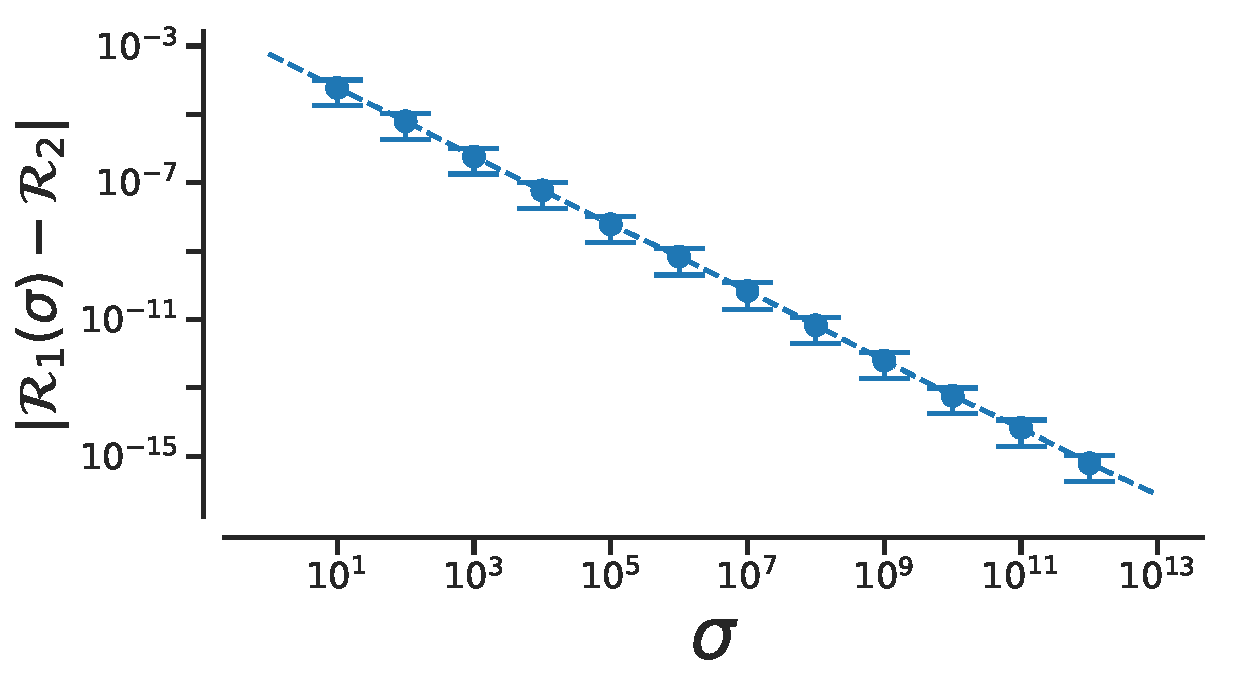
\includegraphics[width=0.6\linewidth]{backmap_fig13.pdf}
\caption{The increase in the acccuracy measure ($\sigma$) for the original Ramachandran number (\Eqn{ramachandran_raw}) results in values that tend towards the new Ramachandran number proposed in this paper (\Eqn{eqn:rama}).\label{fig:sigma}} 
\end{figure} 

Here, $\round{x}$ rounds $x$ to the closest integer value, $\sigma$ is a scaling factor, discussed below, and $\lambda$ is the range of an angle in degrees (i.e., $\lambda=\phi_{\rm max}-\phi_{\rm min}$). Effectively, this equation does the following. \textbf{1)} It divides up the Ramachandran plot into $(360^\circ \sigma^{1/\circ})^2$  squares, where $\sigma$ is a user-selected scaling factor that is measured in reciprocal degrees [see Fig.~8b in \cite{Mannige2016}]. \textbf{2)} It then assigns integer values to each square by setting the lowest integer value to the bottom left of the Ramachandran plot ($\phi=-180^\circ,\psi=-180^\circ$) and proceeding from the bottom left to the top right by iteratively slicing down -1/2 sloped lines and assigning increasing integer values to each square that one encounters. \textbf{3)} Finally, the equation assigns any $(\phi,\psi)$ pair within $\phi,\psi \in [-\phi_{\rm min},\phi_{\rm max})$ to the integer value ($R_\mathbb{Z}$) assigned to the divvied-up square that they it exists in.

Combining the two equations (\Eqns{rama} and \ref{ramachandran_raw}) results in the following, rather imposing, equation for the Ramachandran number:
\begin{equation}
{\mathcal{R}}(\phi,\psi) = 
\frac{
    \left(
	\begin{array}{c c}
	\round{(\phi - \psi + \lambda)\sigma/\sqrt{2}}  
	&    + \round{\sqrt{2} \lambda\sigma} \round{(\phi+\psi + \lambda)\sigma/\sqrt{2}} \\
		 - \round{(\phi_{\rm{min}} - \psi_{\rm{min}} + \lambda)\sigma/\sqrt{2}}  
	&    - \round{\sqrt{2} \lambda\sigma} \round{(\phi_{\rm{min}}+\psi_{\rm{min}} + \lambda)\sigma/\sqrt{2}}
	\end{array}
	\right)\\
 }{
    \left(
	\begin{array}{c c}
	\round{(\phi_{\rm{max}} - \psi_{\rm{max}} + \lambda)\sigma/\sqrt{2}}  
	& + \round{\sqrt{2} \lambda\sigma} \round{(\phi_{\rm{max}}+\psi_{\rm{max}} + \lambda)\sigma/\sqrt{2}}\\
	- \round{(\phi_{\rm{min}} - \psi_{\rm{min}} + \lambda)\sigma/\sqrt{2}}  
	& - \round{\sqrt{2} \lambda\sigma} \round{(\phi_{\rm{min}}+\psi_{\rm{min}} + \lambda)\sigma/\sqrt{2}}
	\end{array}
	\right)
} \label{rama_old}
\end{equation}

However useful \Eqn{rama_old} is, the complexity of the equation may be a deterrent towards utilizing it. This paper reports a simpler equation that is derived by taking the limit of \Eqn{rama_old} as $\sigma$ tends towards $\infty$. In particular, when $\sigma\to\infty$, \Eqn{rama_old} becomes
\begin{equation}
{\mathcal{R}}(\phi,\psi) = \lim_{\sigma\to\infty}{\bar{\mathcal{R}}}(\phi,\psi) = \frac{\phi+\psi-(\psi_{\rm min}+\psi_{\rm min})}{(\phi_{\rm max}+\psi_{\rm max})-(\phi_{\rm min}+\psi_{\rm min})}.
\label{ramaGeneral}
\end{equation}

Assuming that $\phi,\psi \in [-180^\circ,180^\circ)$ or $[-\pi,\pi)$,

\begin{equation}
\mathcal{R}(\phi,\psi) = \frac{\phi+\psi+2\pi}{4\pi}.
\label{rama2}
\end{equation}

Conformation of this limit is shown numerically in \Fig{fig:sigma}. Since larger $\sigma$s indicate higher accuracy, $\displaystyle\lim_{\sigma\to\infty}{\mathcal{R}}(\phi,\psi)$ represents an exact representation of the Ramachandran number. Using this closed form, this report shows how both static structural features and complex structural transitions may be identified with the help of Ramachandran number-derived plots.

Assuming, a different range (say, $\phi,\psi \in [0,2\pi)$), the Ramachandran number in that frame of reference will be
\begin{equation}
{\mathcal{R}}(\phi,\psi)_{\phi,\psi \in [0,2\pi)} = \frac{\phi+\psi}{4\pi}.
\label{ramaGeneral}
\end{equation}
However, in changing the ranges, the meaning of the Ramachandran number will change. This manuscript assumes that all angles ($\phi$,$\psi$,$\omega$) range between $-\pi$ ($-180^\circ$) and $\pi$ ($180^\circ$)

\bibliography{all}


\end{document}
